\documentclass[12pt, twoside]{article}
\usepackage[utf8]{inputenc}
\usepackage[english,russian]{babel}
\newcommand{\hdir}{.}

\usepackage{graphicx}
\usepackage{caption}
\usepackage{amssymb}
\usepackage{mathrsfs}
\usepackage{euscript}
\usepackage{upgreek}
\usepackage{array}
\usepackage{theorem}
\usepackage{graphicx}
\usepackage{subfig}
\usepackage{caption}
\usepackage{color}
\usepackage{url}
\usepackage{amsmath}

\usepackage[left=2cm, right=2cm, top=3cm, bottom=3cm, bindingoffset=0cm]{geometry}

\newcommand{\Pb}{\mathcal{P}}

\setcounter{secnumdepth}{-1}

\begin{document} 

\title{Задание 1 по курсу "Байесовский выбор модели"}
\author{Грабовой Андрей, группа 574}
\date{}
\maketitle

\section{Задача 1}
Пусть проводиться эксперимент по угадыванию стороны выпадения честной монеты. Известно, что оракул прав с вероятностью $p_1 = 0.9$, а обычный человек с вероятностью $p_2 = 0.5$. Известно, что человек $P$ оказался прав во всех n=10 бросаниях. С какой вероятностью $P$ является оракулом, если случайный человек оказывается оракулом с вероятностью $p_a = 10^{-4}$?

Пусть $A = [P - \text{оракул}]$, $B = [n~\text{из}~n]$ - обозначения из лекциии. 

$$\Pb(A|B) = \frac{\Pb(B|A)\Pb(A)}{\Pb(B|\bar{A})\Pb(\bar{A}) + \Pb(B|A)\Pb(A)}, \eqno(1)$$
где $\Pb(A) = 0.0001$, $\Pb(\bar{A}) = 0.9999$.

Подставляя числа в формулу (1) получаем:
$$\Pb(A|B) = \frac{0.9^{10}\cdot10^{-4}}{0.9^{10}\cdot10^{-4} + 0.5^{10}\cdot0.9999} = 0.0345$$

Пусть человек $P$ выбран не случайно, а как лучший среди 100 человек по угадыванию $k = 100$ выпадений монеты. Вывести новую априорную вероятность того, что $P$ оракул с учетом его неслучайного выбора.


Аналитически: Найдем вероятность того, что лучший из 100 это оракул:
$$\Pb(A|C) = \sum_{i=0}^{100}\Pb(A|C, C_O = i)\Pb(C_O = i), \eqno(2)$$
где $C_O$ это случайная величина --- количества оракулов среди 100 человек, $C$ - это событие, что $P$ лучший из 100 человек. Из суммы останется только первых два слагаемых, так как остальные слагаемые будут много меньше:
$$
\Pb(C_O = i) = C_k^ip_a^i(1-p_a)^{k-i} = 
 \begin{cases}
   0.9900 &i=0\\
   0.0099 & i = 1\\
   0.0001 & i = 2
 \end{cases}, \eqno(3)$$
 как видно из (3) нам важны только первые два слагаемых. Получаем:
$$\Pb(A|C) = \Pb(A|C, C_O = 0)\Pb(C_O = 0) + \Pb(A|C, C_O = 1)\Pb(C_O = 1), \eqno(4)$$

Найдем по формуле Байеса $\Pb(A|C, C_O = 0)$ и $\Pb(A|C, C_O = 1)$. 
$$\Pb(A|C, C_O = 0) = \frac{\Pb(C|A, C_O = 0)\Pb(A|C_O = 0)}{\Pb(C|\bar{A}, C_O = 0)\Pb(\bar{A}|C_O = 0) + \Pb(C|A, C_O = 0)\Pb(A|C_O = 0)} = 0, \eqno(5)$$

$$\Pb(A|C, C_O = 1) = \frac{\Pb(C|A, C_O = 1)\Pb(A|C_O = 1)}{\Pb(C|\bar{A}, C_O = 1)\Pb(\bar{A}|C_O = 1) + \Pb(C|A, C_O = 1)\Pb(A|C_O = 1)}, \eqno(6)$$

Найдем вероятность того, что оракул "проиграет" простому человеку при  $k>>1$. При $k>>1$ биномиальную случайную величину можно приблизить нормальной случайной величиной, тоесть:
$$\Pb(\text{оракул проиграл}) = \Pb(O < H) = \int_{-\infty}^{\infty} \Pb(O < t) p_{N_2}(t)dt = 
\int_{-\infty}^{\infty} p_{N_2}(t) \int_{-\infty}^{t} p_{N_1}(\omega)d\omega dt = $$
$$= \frac{1}{2}\int_{-\infty}^{\infty} p_{N_2}(t) [\text{erf}\left(\frac{t - p_1k}{\sqrt{2p_1(1-p_1)k}}\right) + 1]dt$$
где $N_2 = N(p_2k, p_2(1-p_2)k),~ N_1 = N(p_1k, p_1(1-p_1)k)$

\begin{figure}[h!]\center
{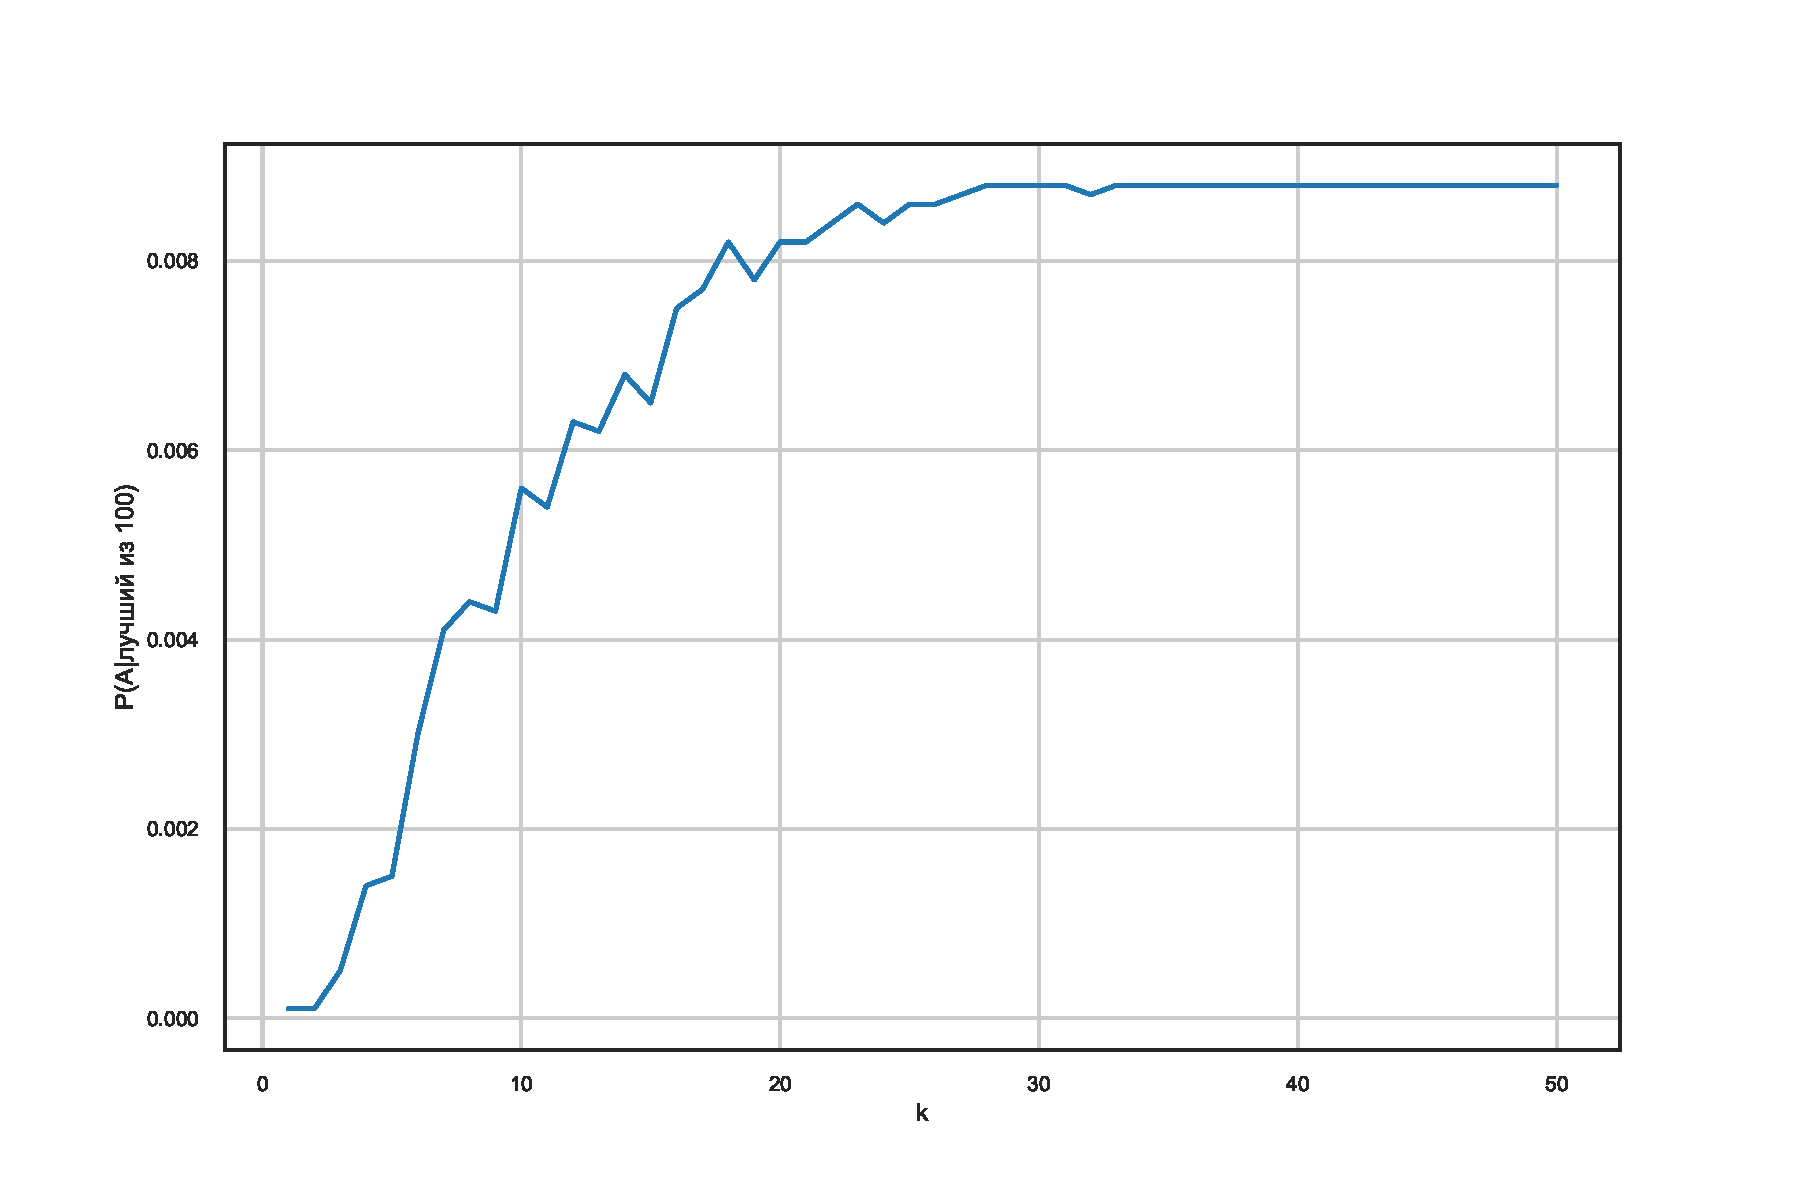
\includegraphics[width=0.8\textwidth]{sampler_task1}}
\caption{График зависимости апостериорной вероятности от количества бросаний монеты}
\label{sampler_task1}
\end{figure}

При k = 100 получаем, что $\Pb(\text{оракул проиграл}) = 10^{-14}$. Получаем, что
$$\Pb(C|A,C_O=1)~\approx~1.0, \eqno(7)$$
$$\Pb(C|\bar{A},C_O=1)~\approx~0.0, \eqno(8)$$

Тогда подставляя (7-8) в (6) получаем, что $\Pb(A|C, C_O = 0) \approx 1.0$, откуда получаеться, что
$$\Pb(A|C) \approx 0.01, \eqno(9)$$

Сэмплированием: Сгенерируем выборку учитывая наше априорное представление о модели.
Пусть у нас есть 1000 групп людей по 100 человек, где каждый человек оракул с вероятностью $\Pb(A) = 10^{-4}$. После каждый человек бросает монету $k = 1...50$ раз и в каждой группе получаем ' лучшего' кандидата. После этого смотрим оракул он или нет и получаем апостериорную вероятность что лучший из 100 будет оракулом как частоту. Построим график зависимости $\Pb(A|C)$ от числа $k$.



Из аналитического решения и с сэмплирования Рис.~\ref{sampler_task1}, получаем что~$\Pb(A|C)~\approx~0.01$.

\section{Задача 2}
Пусть имеется i.i.d выборка $\textbf{X} = \{x_1, \cdots x_n\}$ из неизвестного распределения с конечной плотностью. На уровне значимости  $\alpha = 0.05$ проверить гипотезу о том, что деситипроцентная квантиль распределения равна $m_0 = 0$. 

Начальная гипотеза эквивалентная гипотезе о том, что в выборке $10\%$ данных меньше нуля.

Построим статистику:
$$T(\textbf{X}) = \frac{1}{2n}\sum_{i = 1}^{n}(-\text{sign}(x_i) + 1). \eqno(10)$$

По ЦПТ:
$$T(\textbf{X}) \sim N(\tau, \frac{\mathsf{S}^2}{n}), \eqno(11)$$
где $\mathsf{S}^2$ --- это несмещенная выборочная дисперсия выборки $\frac{1}{2}(-\text{sign}(\textbf{X}) + 1)$. 

Тогда получаем, что если $T(\textbf{X}) $ попадает в область закрашенную на Рис.~\ref{sampler_task2_p1}, гипотеза о том, что деситипроцентная квантиль распределения равна $m_0 = 0$ отвергается, в противном случае, если не попадает, то данные не противоречат гипотезе (о том, что $\tau = 0.1$).
\begin{figure}[h!]\center
{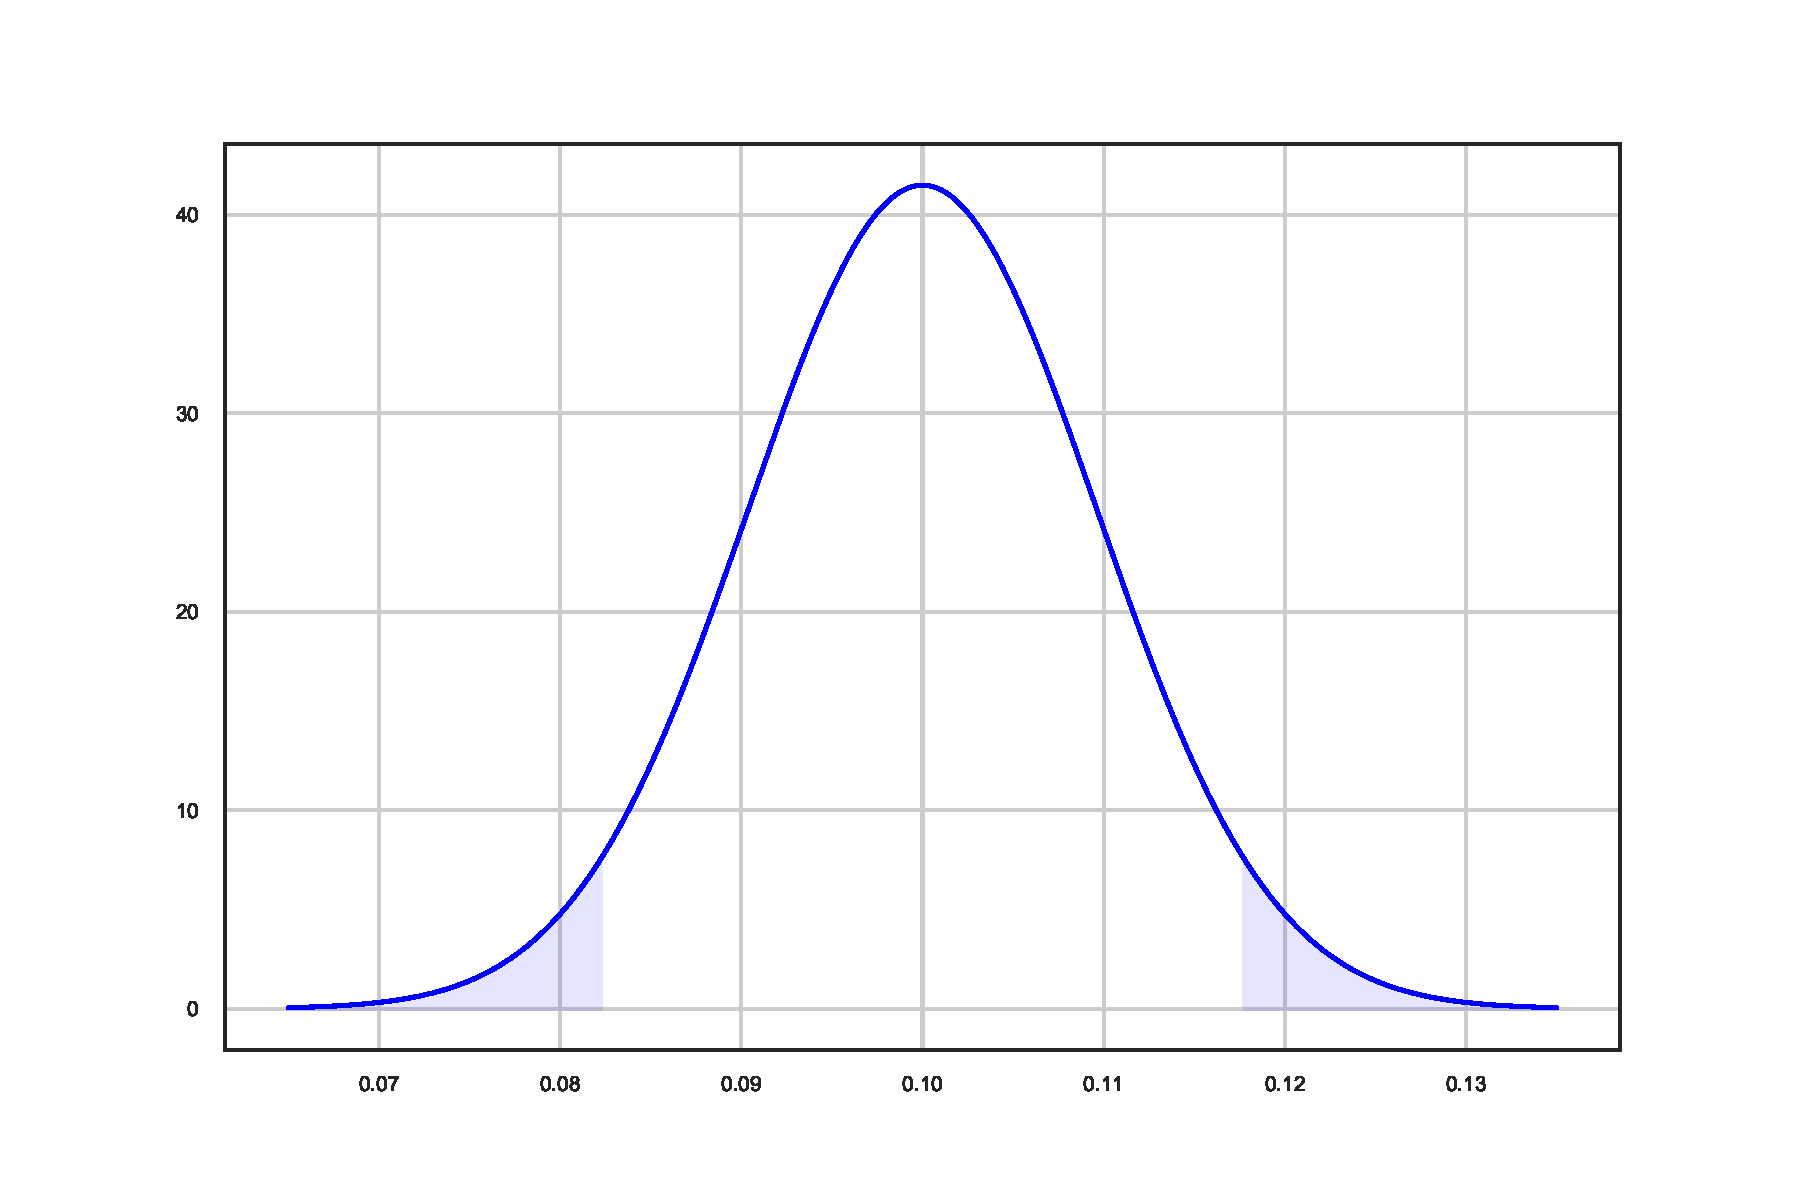
\includegraphics[width=0.8\textwidth]{sampler_task2_p1}}
\caption{График плотности распределения для n = 1000}
\label{sampler_task2_p1}
\end{figure}


\section{Задача 3}
Пусть имеется выборка пар $\textbf{z}_i=(x_i,y_i),~i=1...n$. $\textbf{z}_i \sim N([0,0]^\text{T}, \begin{bmatrix}
1 & \rho\\
\rho & 1\\
\end{bmatrix})$

Для статистики $T_1(\textbf{Z}) = \frac{1}{n}\sum_{i=1}^{n}x_iy_i$, получить плотность распределения. Из ЦПТ получается, что:

$$T_1(\textbf{Z}) \sim N(\rho, \frac{1}{n}), \eqno(12)$$

Тогда для $T_1(\textbf{Z})$ получаем следующий график плотностей распределения:

\begin{figure}[h!]\center
{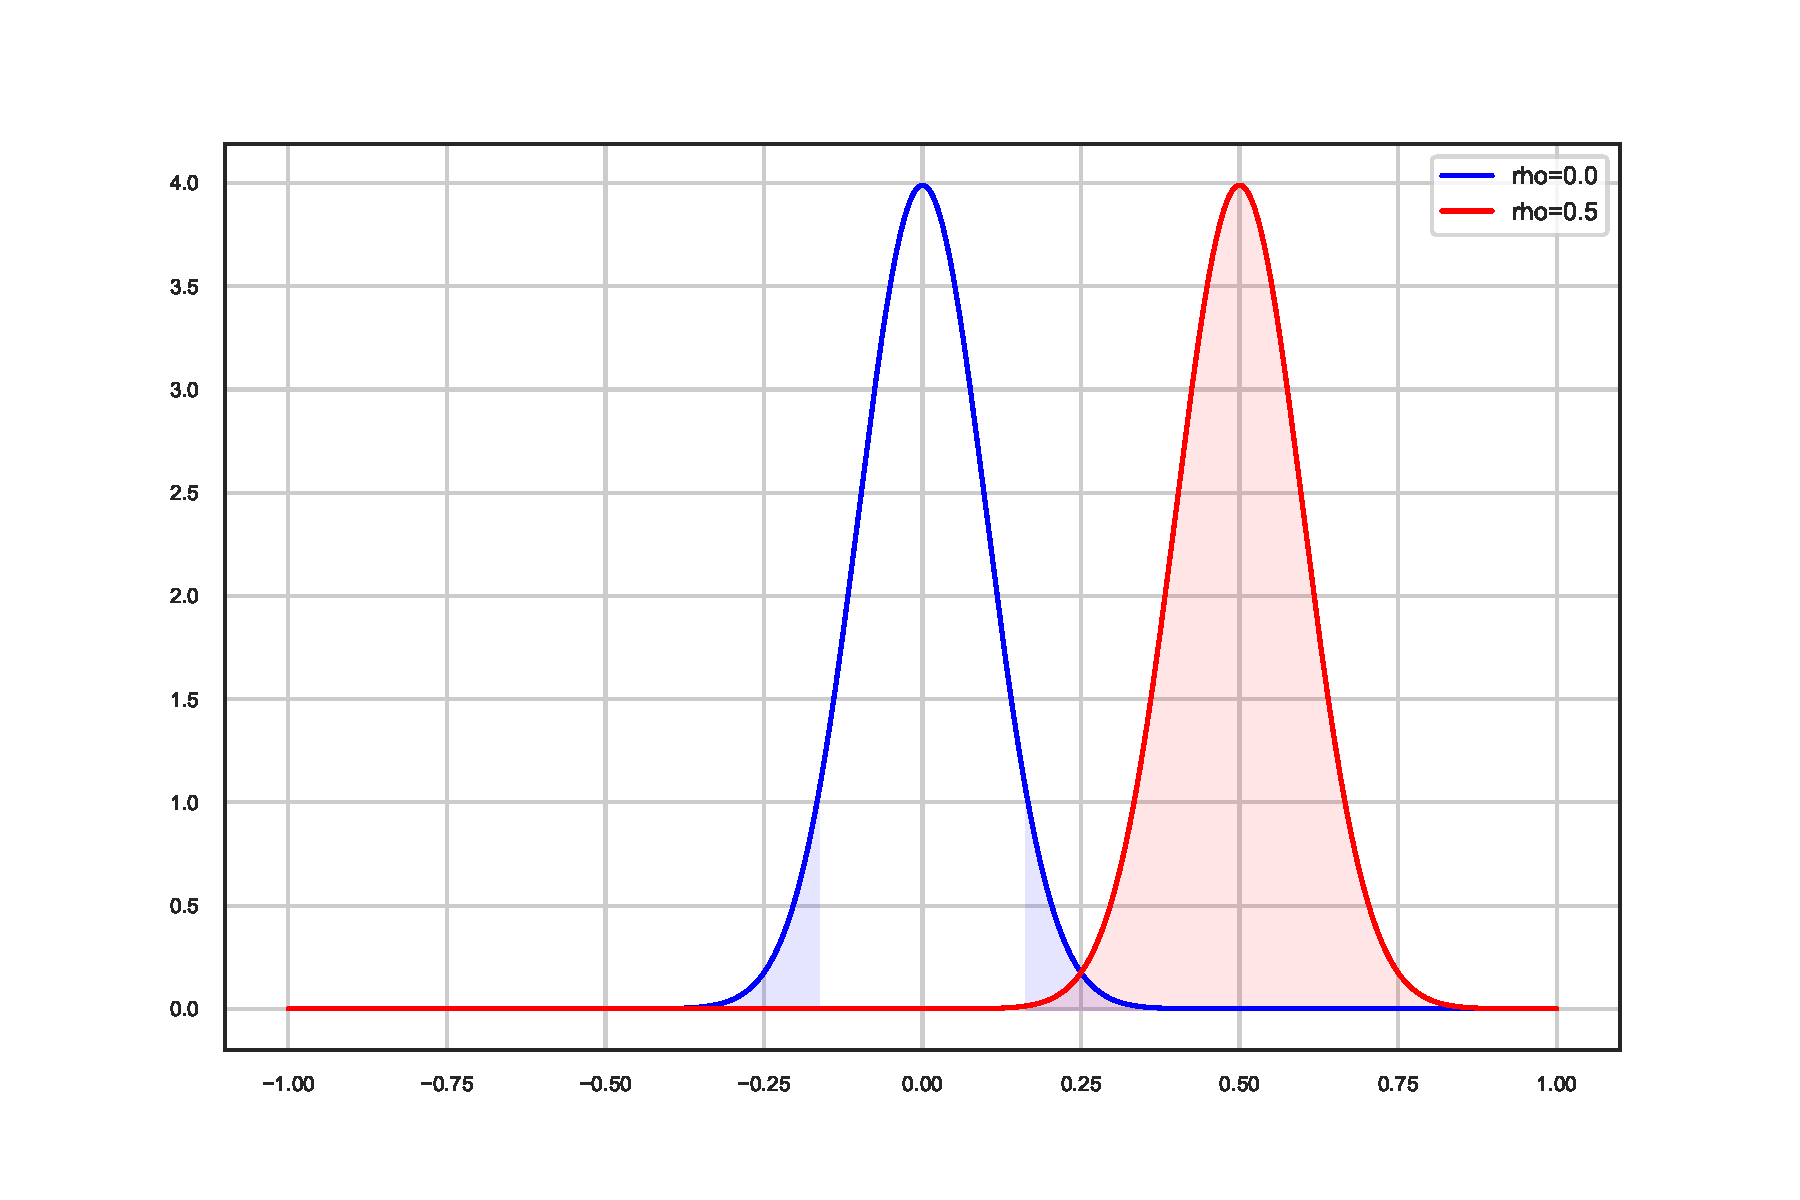
\includegraphics[width=0.8\textwidth]{sampler_task3_p1}}
\caption{График плотностей распределений для разных $\rho$}
\label{sampler_task3_p1}
\end{figure}

\begin{figure}[h!]\center
{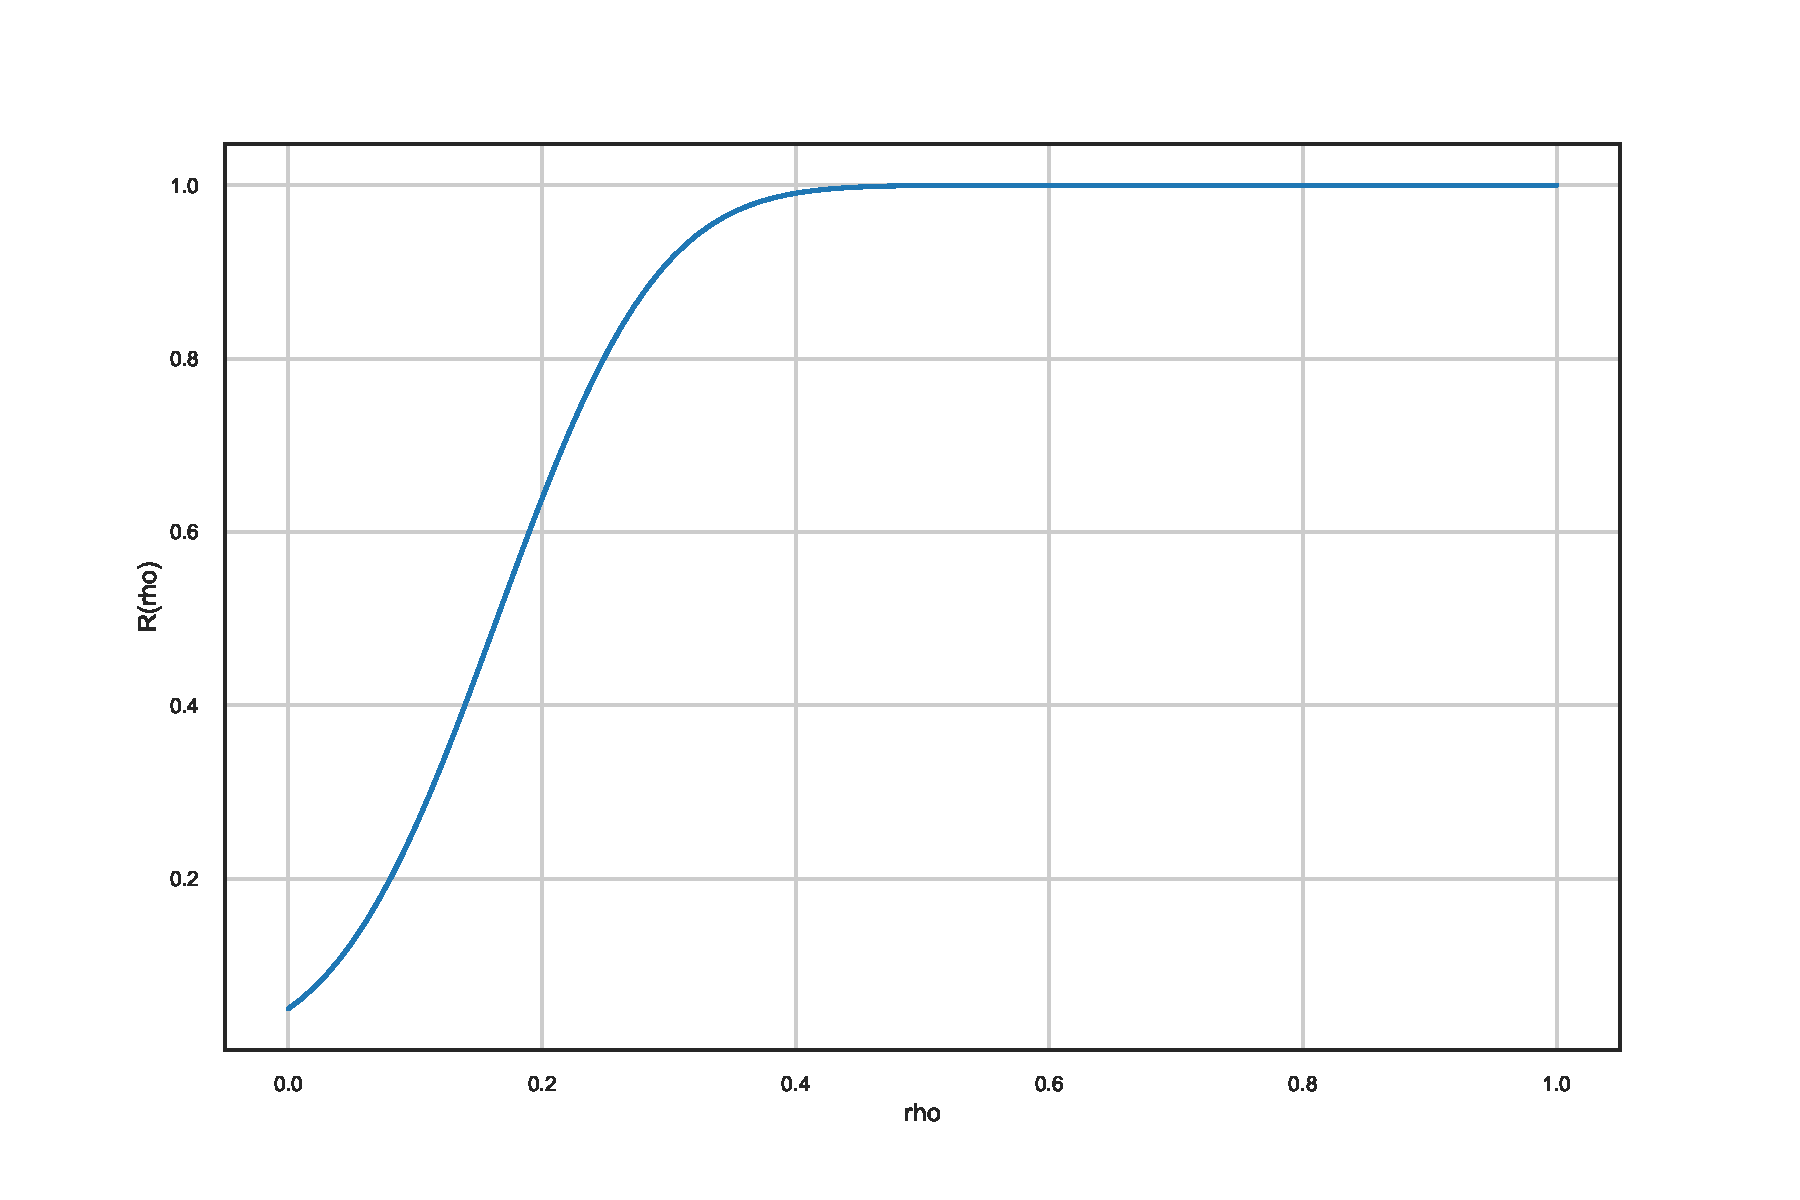
\includegraphics[width=0.8\textwidth]{sampler_task3_p2}}
\caption{График зависимости мощности от $\rho$ аналитически}
\label{sampler_task3_p2}
\end{figure}


Будем проверять гипотезу $H_0$ о том, что $\rho = 0$ на уровне значимости $\alpha = 0.05$.
На Рис.~\ref{sampler_task3_p1} показан мощность критерия для $\rho = 0.5$.

Найдем мощность критерия $R_1(\rho)$ аналитически:

$$R_1(\rho) \approx \int_{0.1645}^{\infty} p_{N(\rho, \frac{1}{n})}(x)dx = \frac{\sqrt{n}}{\sqrt{2\pi}}\int_{a}^{\infty} 
e^{-(\frac{\sqrt{n}x}{\sqrt{2}}-\frac{\sqrt{n}\rho}{\sqrt{2}})^2}dx = $$
$$=\frac{1}{\sqrt{\pi}} \int_{a\frac{\sqrt{n}}{\sqrt{2}}}^{\infty} e^{-(x - \frac{\sqrt{n}\rho}{\sqrt{2}})^2}dx = 
\frac{1}{\sqrt{\pi}} \int_{a - \frac{\sqrt{n}\rho}{\sqrt{2}}}^{\infty} e^{-x^2}dx = \frac{1}{2}\text{erfc}\left((0.1645 - \rho)\sqrt{\frac{n}{2}}\right), \eqno(13)$$


\begin{figure}[h!]\center
{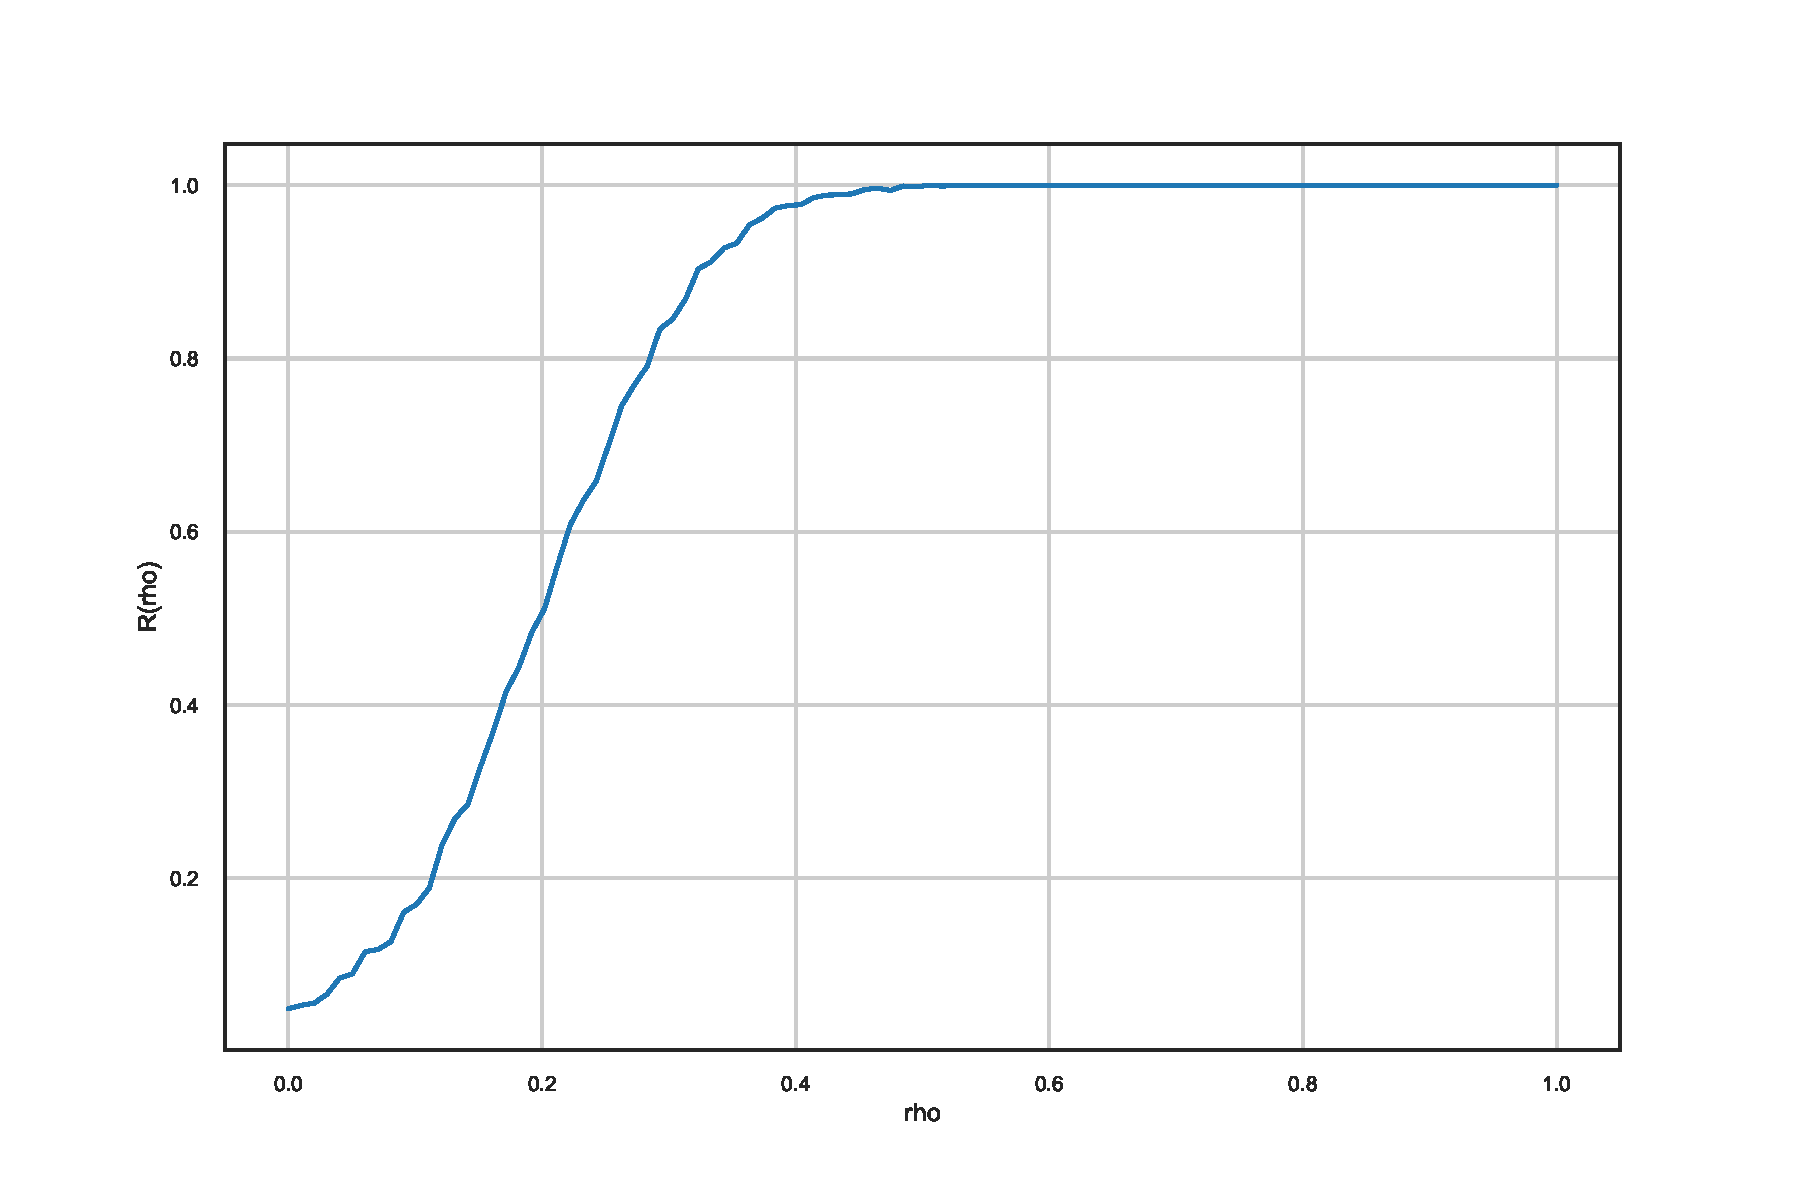
\includegraphics[width=0.8\textwidth]{sampler_task3_p3}}
\caption{График зависимости мощности от $\rho$ сэмплированием}
\label{sampler_task3_p3}
\end{figure}

На Рис.~\ref{sampler_task3_p2} показан график зависимости мощности критерия $R_1(\rho)$ найденый аналитически. На Рис.~\ref{sampler_task3_p3} показан график зависимости мощности критерия $R_1(\rho)$ найденый сэмплиированиием.

Сравнить мощность в зависимости от $\rho$ со статистикой $T_2(\textbf{Z}) = \frac{1}{2n}\sum_{i=1}^{n}(x_i - y_i)^2$, рассмотренной на лекции.

Для статистики $T_2(\textbf{Z}) = \frac{1}{2n}\sum_{i=1}^{n}(x_i - y_i)^2$, из ЦПТ получается, что:

$$T_2(\textbf{Z}) \sim N(1-\rho, \frac{(1-\rho)^2}{n}), \eqno(14)$$

Тогда для $T_2(\textbf{Z})$ получаем график плотностей распределения показанный на Рис.~\ref{sampler_task3_p4}.

\begin{figure}[h!]\center
{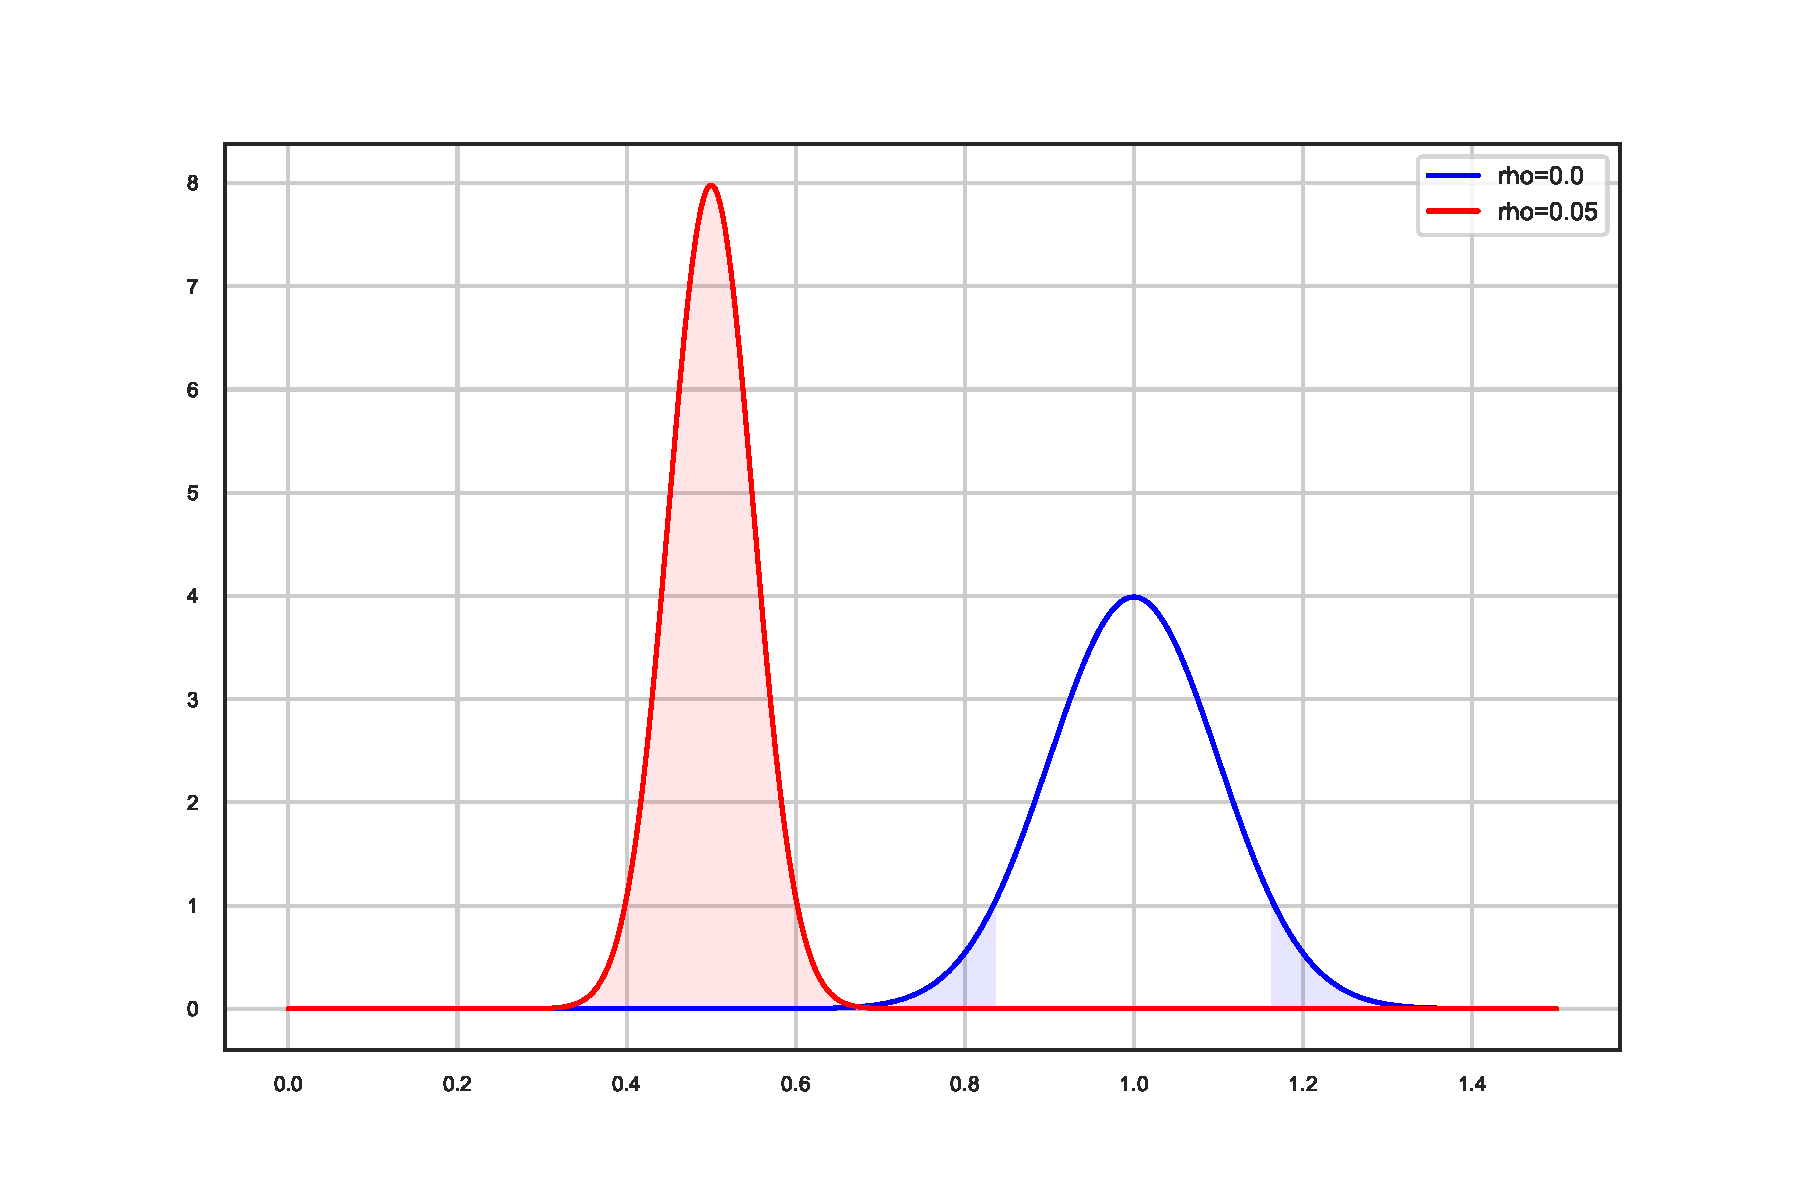
\includegraphics[width=0.8\textwidth]{sampler_task3_p4}}
\caption{График плотностей распределений для разных $\rho$}
\label{sampler_task3_p4}
\end{figure}

Будем проверять гипотезу $H_0$ о том, что $\rho = 0$ на уровне значимости $\alpha = 0.05$.
На Рис.~\ref{sampler_task3_p4} показан мощность критерия для $\rho = 0.5$.

Найдем мощность критерия $R_2(\rho)$ аналитически:

$$R_2(\rho) \approx \int_{-\infty}^{0.8355} p_{N(1-\rho, \frac{(1-\rho)^2}{n})}(x)dx = \frac{\sqrt{n}}{\sqrt{2\pi}(1-\rho)}\int_{-\infty}^{a}
e^{-(\frac{\sqrt{n}x}{\sqrt{2}(1-\rho)}-\frac{\sqrt{n}}{\sqrt{2}})^2}dx = $$
$$=\frac{1}{\sqrt{\pi}} \int_{-\infty}^{a\frac{\sqrt{n}}{\sqrt{2}(1-\rho)}} e^{-(x - \frac{\sqrt{n}}{\sqrt{2}})^2}dx = 
\frac{1}{\sqrt{\pi}} \int_{-\infty}^{a\frac{\sqrt{n}}{\sqrt{2}(1-\rho)}-\frac{\sqrt{n}}{\sqrt{2}}}  e^{-x^2}dx = \frac{1}{2}\text{erf}\left((\frac{0.8355}{1-\rho} - 1)\sqrt{\frac{n}{2}}\right) +\frac{1}{2}, \eqno(15)$$

\begin{figure}[h!]\center
{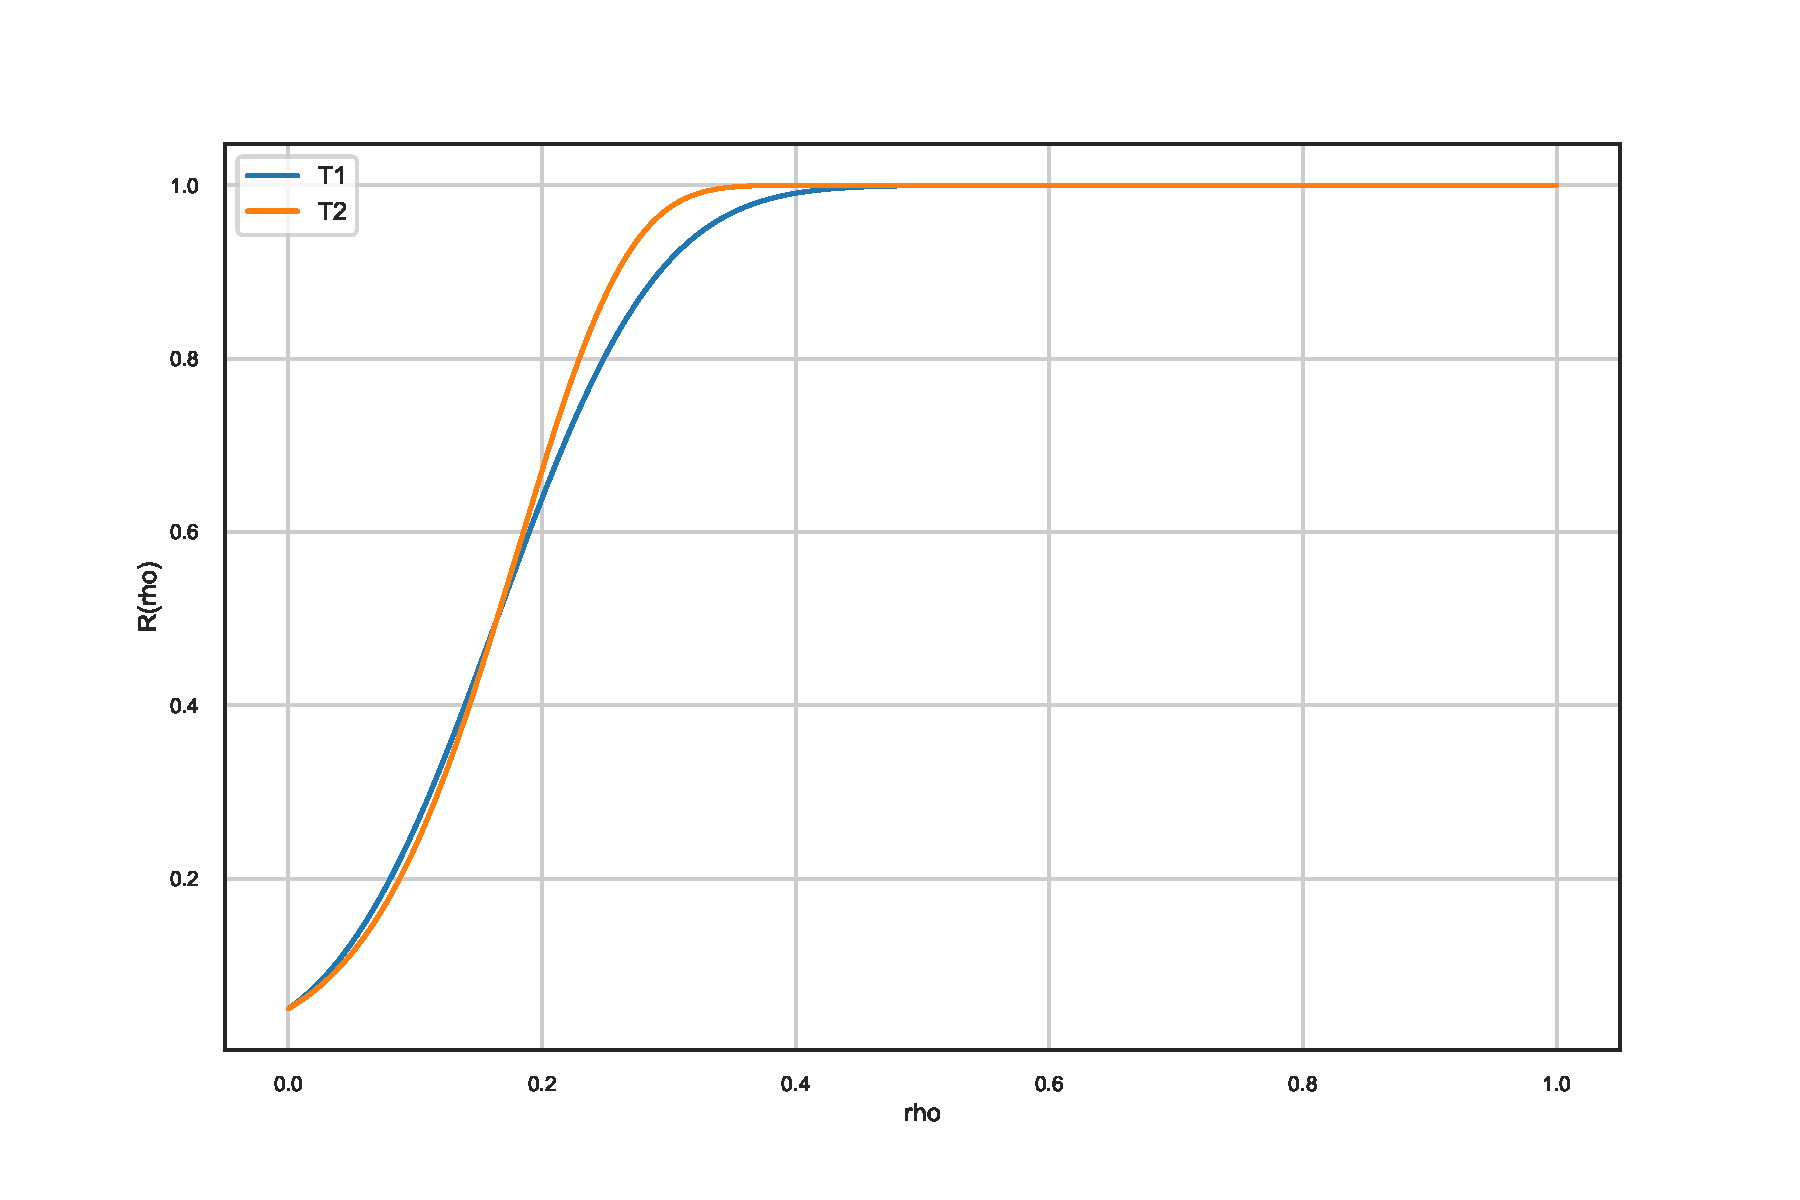
\includegraphics[width=0.8\textwidth]{sampler_task3_p5}}
\caption{График зависимости мощности от $\rho$ для разных статистик}
\label{sampler_task3_p5}
\end{figure}

Как видно из Рис.~\ref{sampler_task3_p5} статистика $T_2(\textbf{Z})$ лучше чем статистика $T_1(\textbf{Z})$, так-как график мощности лежит выше.

\begin{figure}[h!]\center
{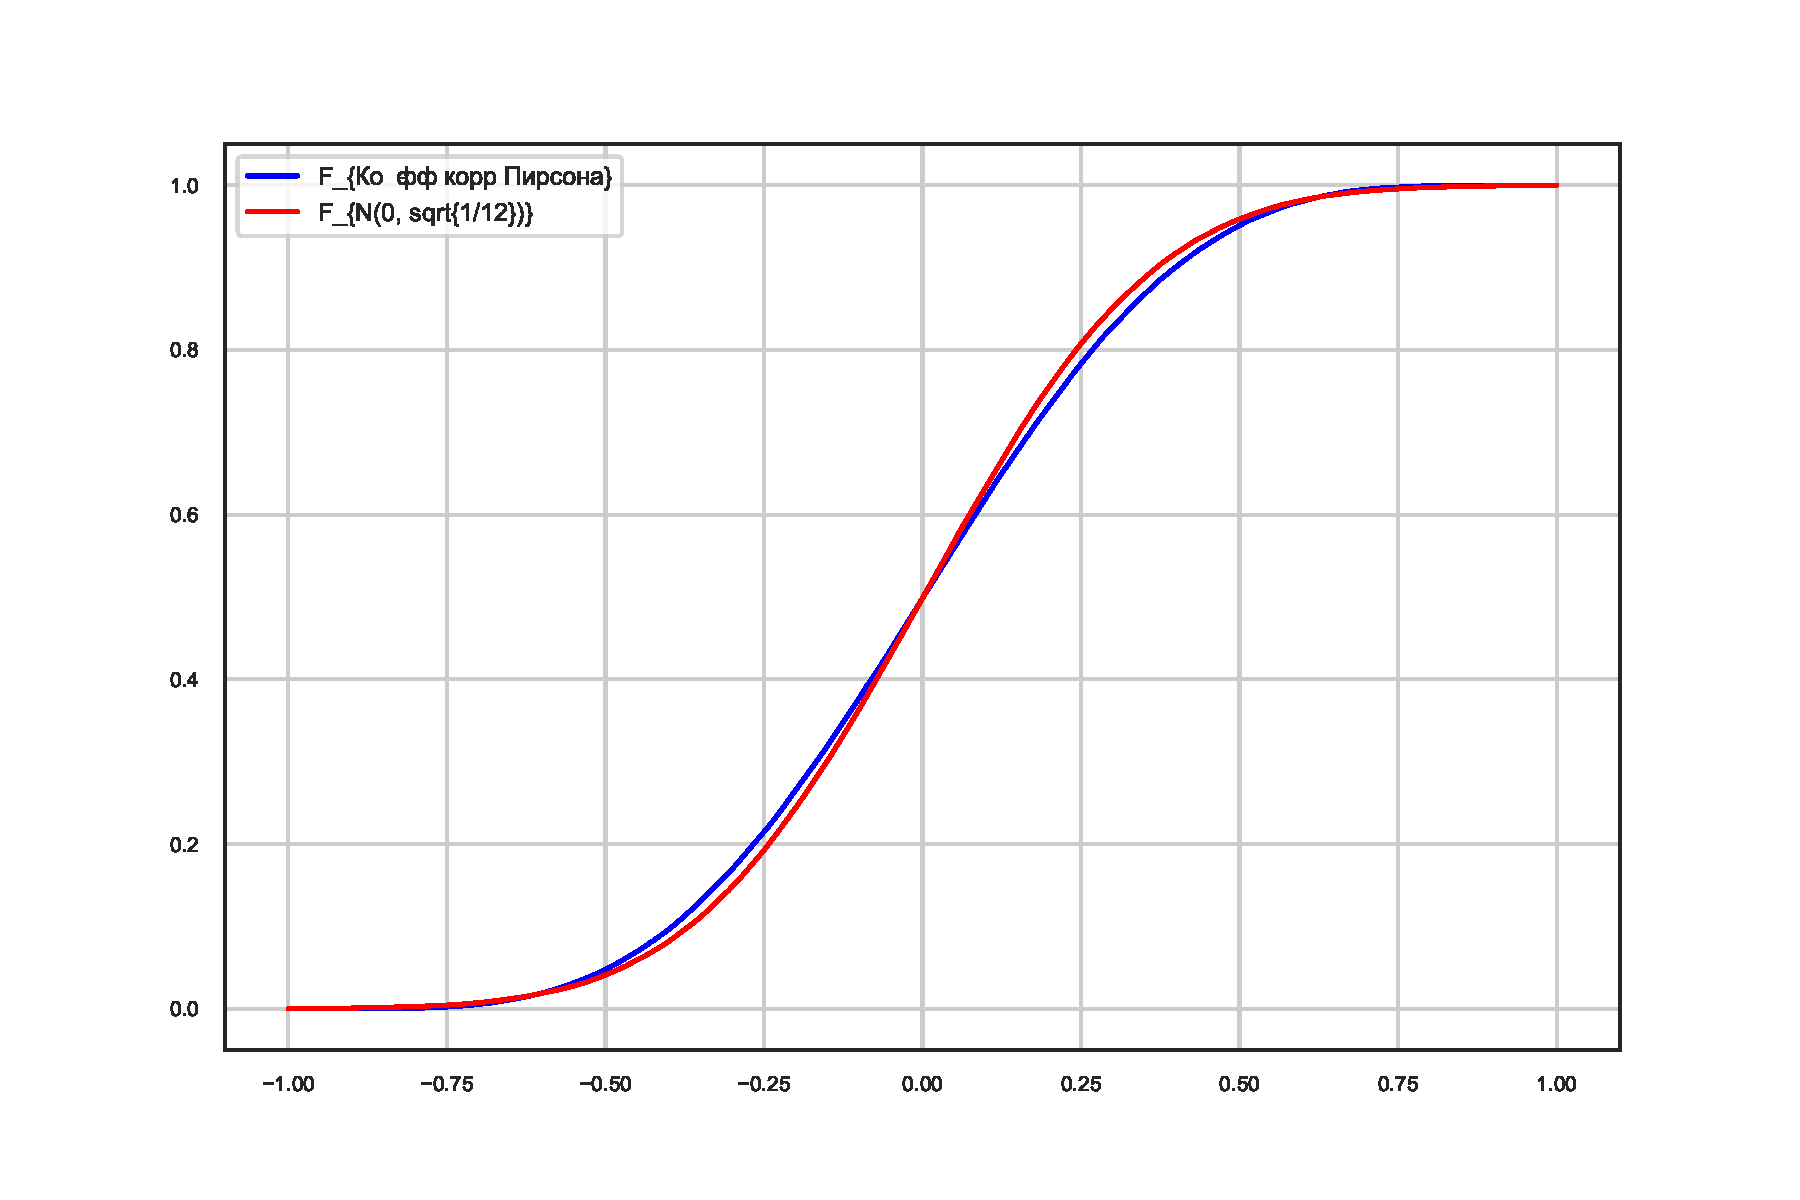
\includegraphics[width=0.8\textwidth]{sampler_task4_p1}}
\caption{Функции распределения $N(0, \frac{1}{12})$ и распределения корр. коэф. Пирсона}
\label{sampler_task4_p1}
\end{figure}

\section{Задача 4}
Пусть $\textbf{x} = \{x_1, \cdots x_n\},~n=12$ есть i.i.d выборка из $N(0,1)$. Пусть $\textbf{y} = \{y_1, \cdots y_n\},~n=12$ есть i.i.d выборка из $N(0,1)$, независимая от $\textbf{x}$. Оценить, сколько разных $K$выборок $\textbf{y}$ нужно рассмотреть, чтобы найти ту, которая дает выборочную корреляцию с $\textbf{x}$ не менее $\rho = 0.97$

Заметим, что распределение выборочной корреляции это $N(0, \frac{1}{12})$, в чем можно убедиться с Рис.~\ref{sampler_task4_p1} на котором изображена эмпирическая функция распределения данных и функция распределения $N(0, \frac{1}{12})$

Учитывая нормальность распределения, получаем, что $\Pb_{N(0, \frac{1}{12})}(x > 0.97) = 10^{-4}$. Математическое ожидание, времени ожидание пока выпадет $\textbf{y}$ такой что $\rho = 0.97$, равно $\mathsf{E}t = 10^4$ (из геометрического распределения).



\begin{figure}[h!]\center
{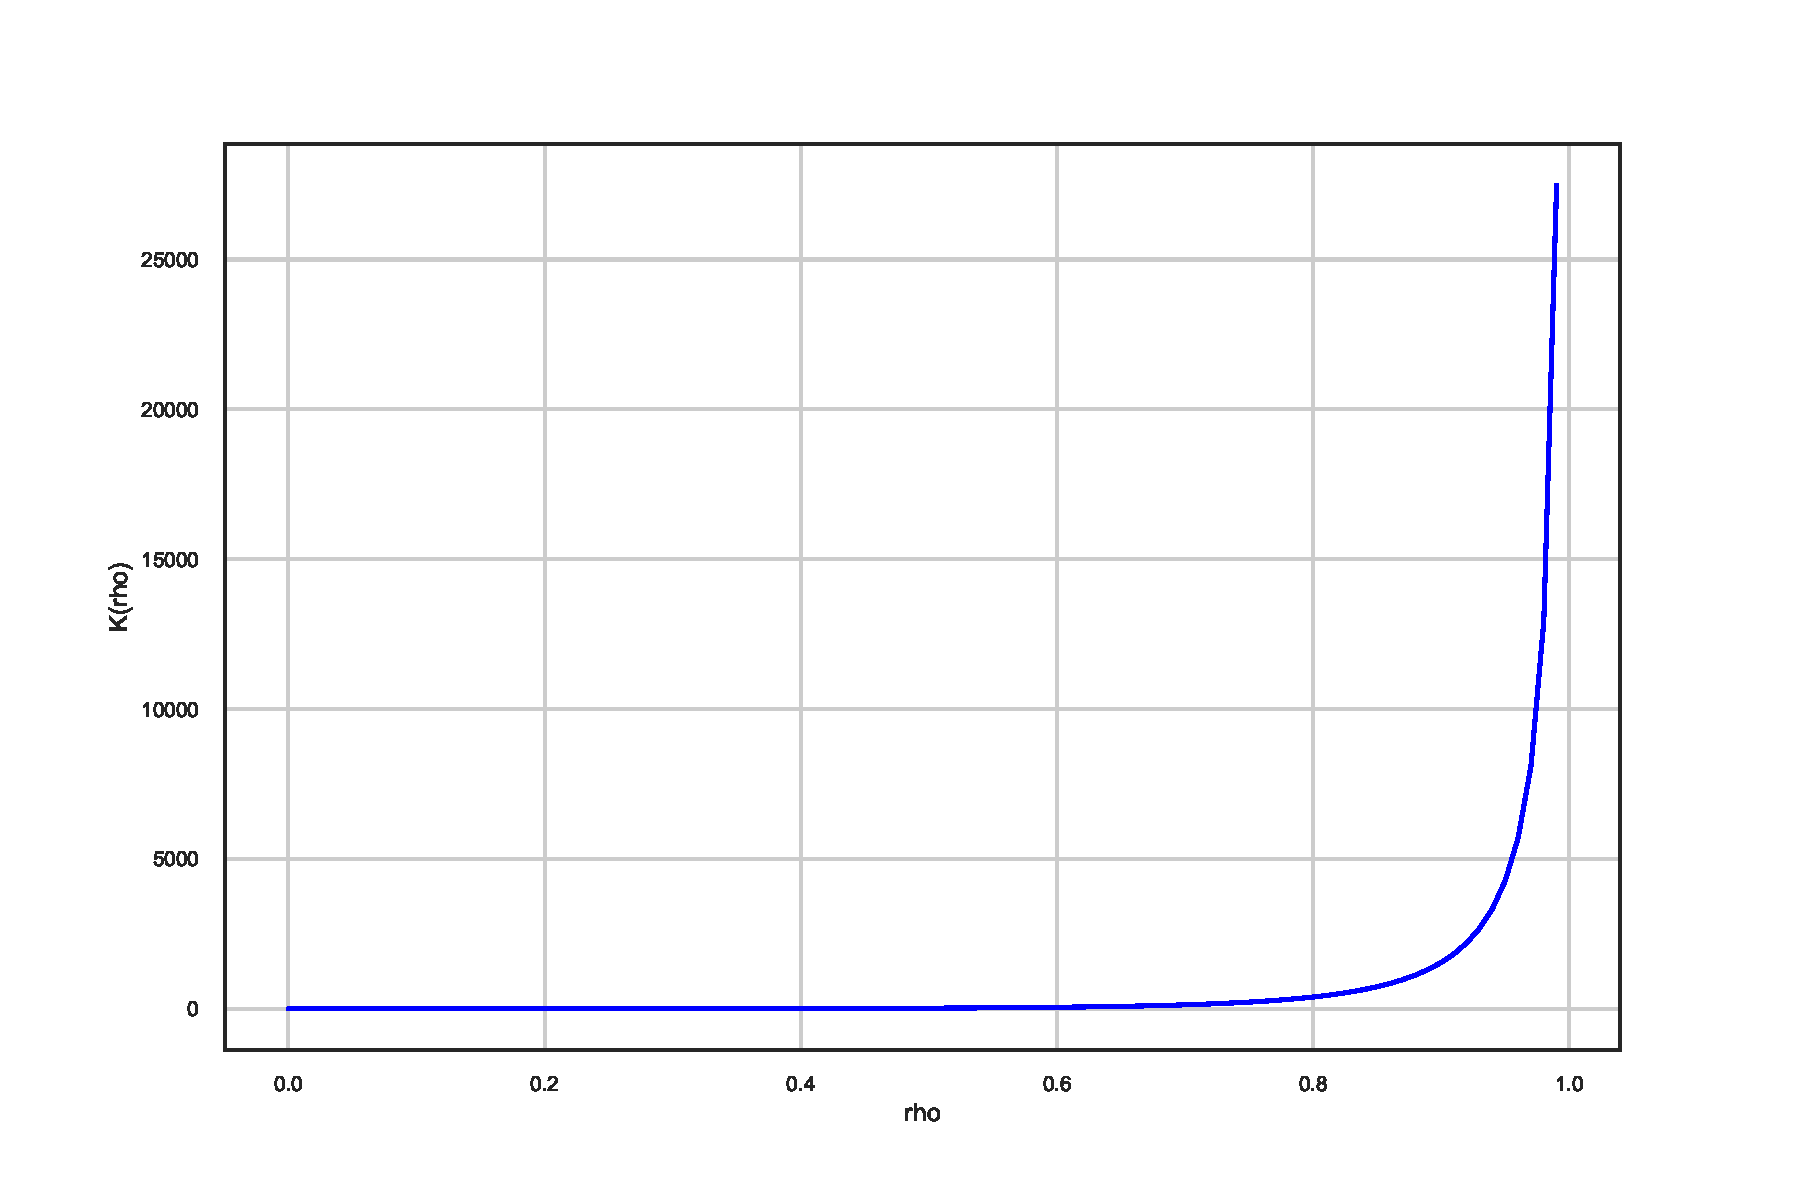
\includegraphics[width=0.8\textwidth]{sampler_task4_p2}}
\caption{График изменения времени ожидания от нужной ковариации}
\label{sampler_task4_p2}
\end{figure}

Построить график зависимости $K(\rho)$ в диапазоне от $0$ до $0.99$.

На Рис.~\ref{sampler_task4_p2} показан зависимости ожидаемого времени ожидания от заданого~$\rho$. 


\section{Задача 5}
Привести пример, когда наивный байесовский классификатор классифицирует объекты не луяше, чем наугад, хотя генеральная совокупность(все возможные объекты) идеально разделимы.

\begin{figure}[h!]\center
{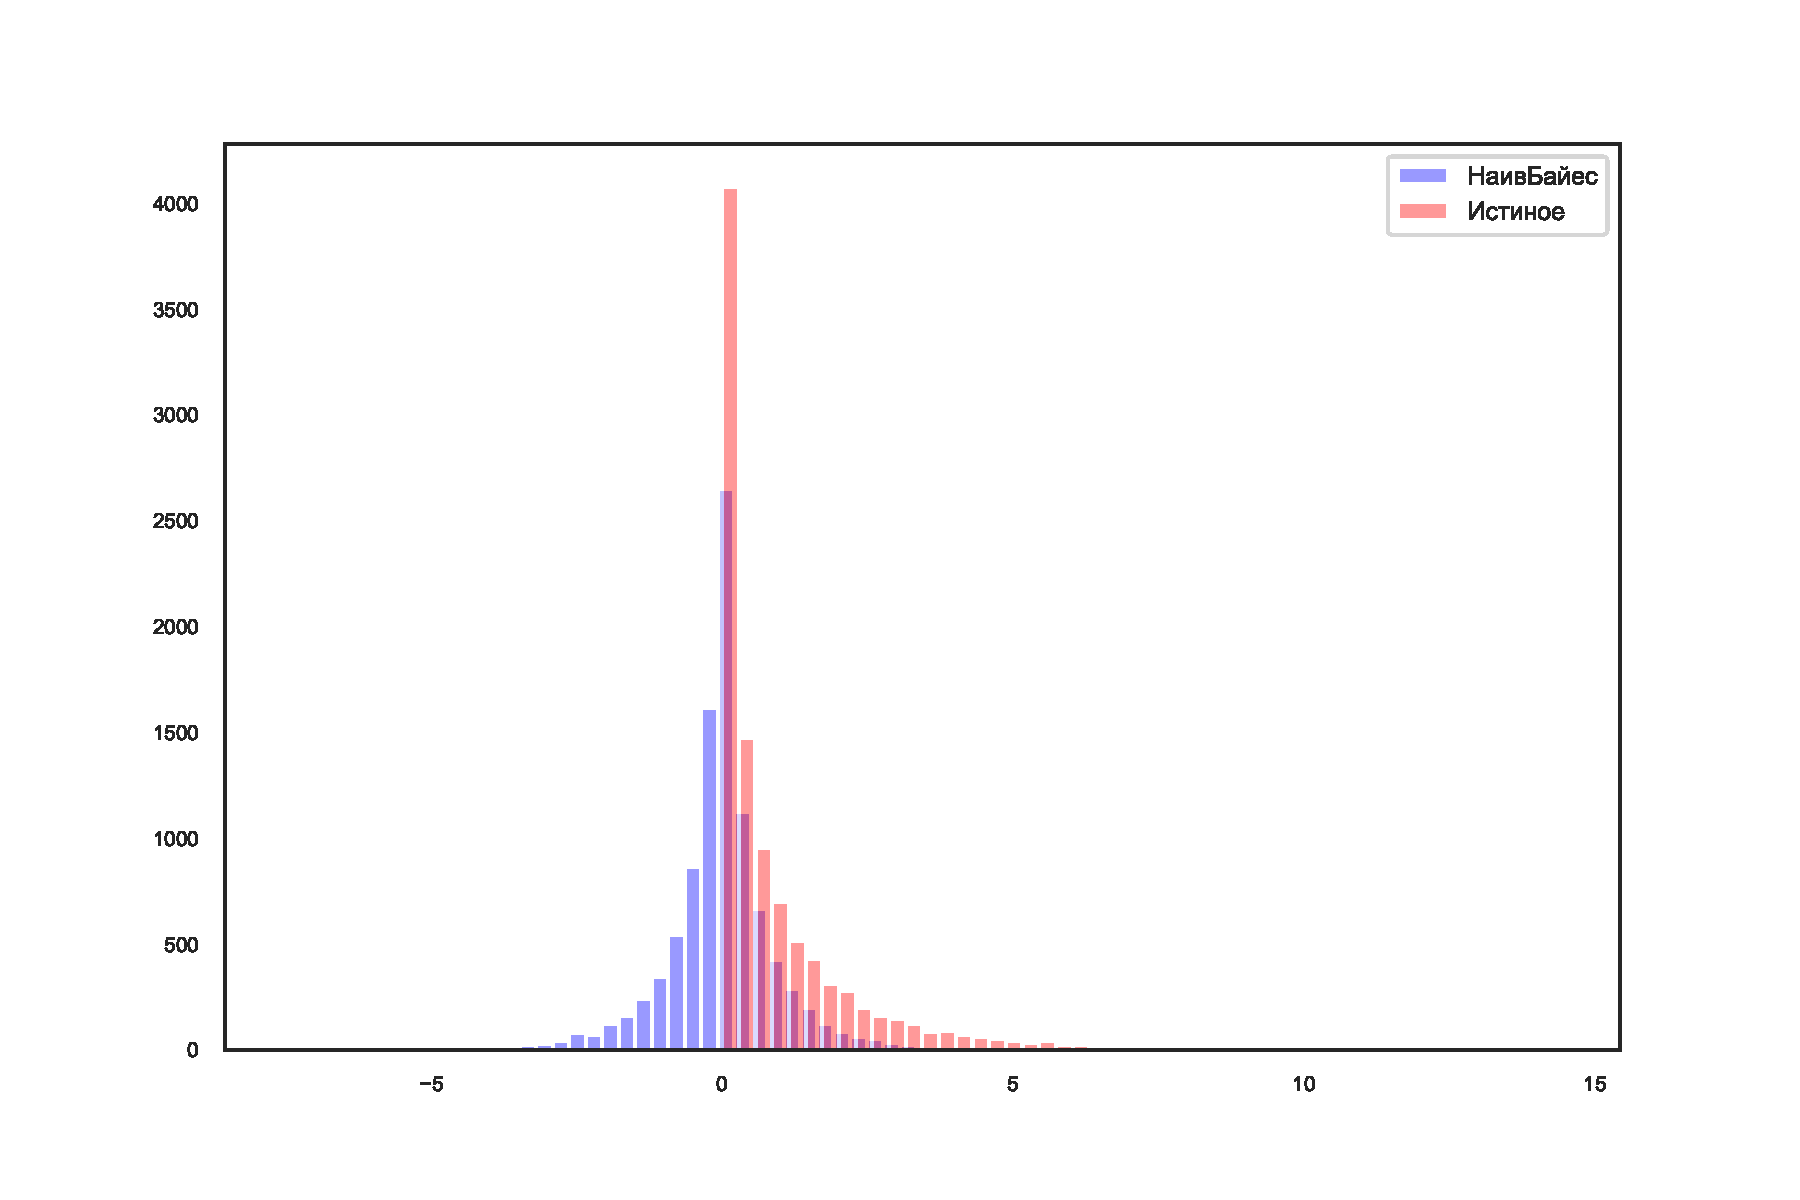
\includegraphics[width=0.8\textwidth]{sampler_task5}}
\caption{Гистаграмма наивного Байеса и истинного распределения}
\label{sampler_task5}
\end{figure}

Рассмотрим выборку распределенную по закону $\textbf{X} = \left\{(x^1_i, x^2_i)^T| (x^1_i, x^2_i) \sim N\left((0, 0)^T, \begin{bmatrix}
1 & 1\\
1 & 1\\
\end{bmatrix}\right)\right\}$, то есть первый и второй признак идеально коррелируемый (то есть просто равен друг другу). Пусть ответом будет знак произведения $y_i = \text{sign}(x^1_ix^2_i)$. 

В силу того, что признаки идеально коррелируемые получим, что все ответы положительные(распределены по $\chi^2$). 

Что же мы получим с точки зрения наивного байесового класификатора. Наивный Байес будет считать что $x^1_i$ и $x^2_i$ независимые и тогда плотность распределения будет симметричная относительно оси ординат, что показано на Рис.~\ref{sampler_task5}. То есть наивный Байес будет классифицировать объекты не лучше чем наугад.

\section{Задача 6}

В услувиях задачи 3 для $\rho = 0.2$ и $\rho=0.0$ при $n=100$, сэмплировать $m = 1000$ выборок пар $z_i, i=1...m$. С помощью статистики $T(\textbf{Z}) = \frac{1}{n}\sum_{i=1}^{n}x_iy_i$ получить достигнутые уровни значимости $p_1, \cdots p_m$. 

\begin{figure}[h!]\center
{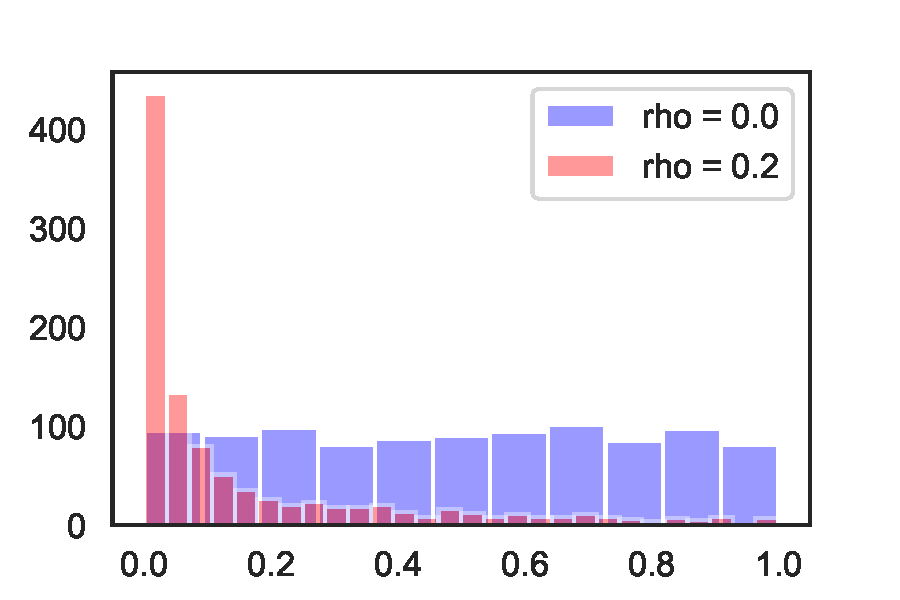
\includegraphics[width=0.8\textwidth]{sampler_task6_p2}}
\caption{Гистограма распределение p-value без поправок}
\label{sampler_task6_p2}
\end{figure}

\begin{figure}[h!]\center
{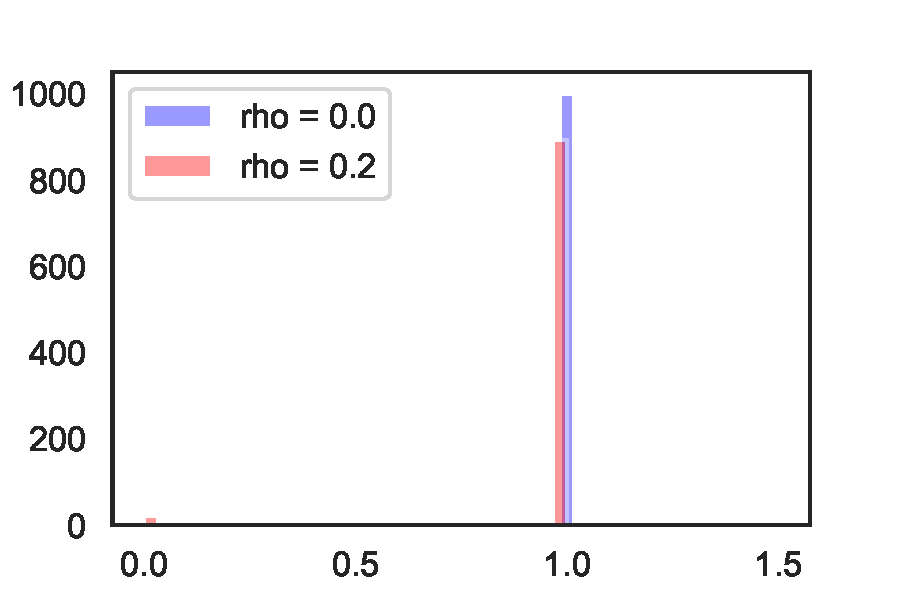
\includegraphics[width=0.8\textwidth]{sampler_task6_p3}}
\caption{Гистограма распределение p-value с Банферонии}
\label{sampler_task6_p3}
\end{figure}

\begin{figure}[h!]\center
{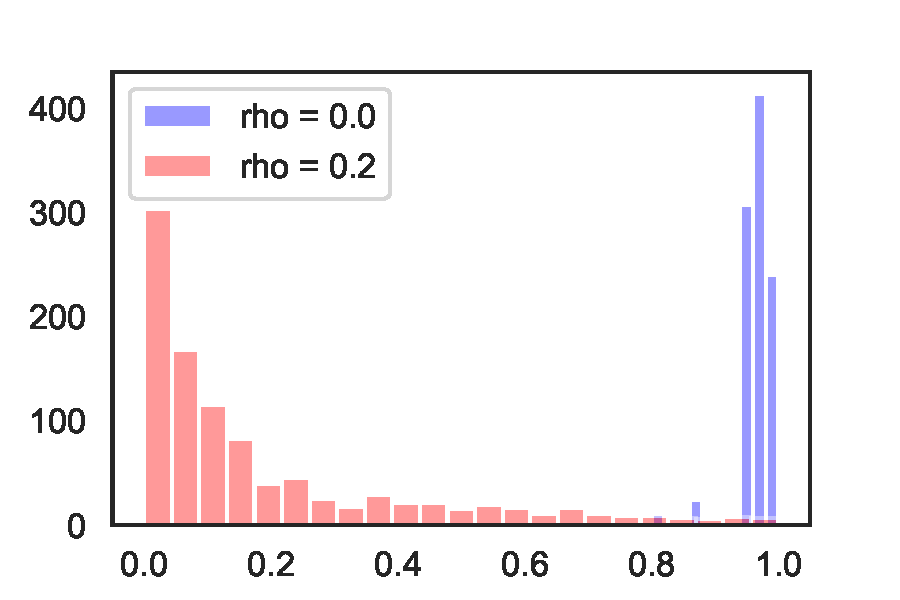
\includegraphics[width=0.8\textwidth]{sampler_task6_p4}}
\caption{Гистограма распределение p-value с Бенджамини-Хохберг}
\label{sampler_task6_p4}
\end{figure}

Распределение достигаемых уровней показаны на Рис.~[\ref{sampler_task6_p2},~\ref{sampler_task6_p3},~\ref{sampler_task6_p4}]


Для уровня значимости $\alpha = 0.05$ сравним результаты применения отсутствия поправки на на множественном тестирование и с использованием поправок Бонферони и Бенджамини-Хохберга. Результаты эксперимента показаны в таб.~\ref{table1}.

\begin{table}[h!]
\begin{center}
\begin{tabular}{|c|c|c|}
\hline
	Метод&Ложно отклоненные& Ложно принятые\\
	\hline
	Без поправки &  93 & 400 \\
	\hline
	Бонферони & 0 & 960\\
	\hline
	Бенджамини-Хохберга& 1 & 517 \\
\hline
\end{tabular}
\end{center}
\caption{Для уровня значимости $\alpha = 0.05$}
\label{table1}
\end{table}

Контролирует ли поправка Бенджамини-Хохберга $FDR$ на уровне $\alpha = 0.05$?
Поправка Бенджамини-Хохберга контролирует $FDR$ на уровне $\alpha = 0.05$, так-как статистики $T_i$ независимые.

\section{Задача 7}
В условиях задачи 6 сэмплировать m = 1000 выборок пар, но с $\rho_m$, зависящее от номера выборки. Провести те же исследования, что и в задаче 6.

$$
\rho_1 = 0, \rho_i = 
 \begin{cases}
   \rho_{i-1}&\text{ с вероятностью 0.3}\\
   0.2 - \rho_{i-1}&\text{ с вероятностью 0.7}
 \end{cases}. \eqno(16)$$
 
 \begin{figure}[h!]\center
{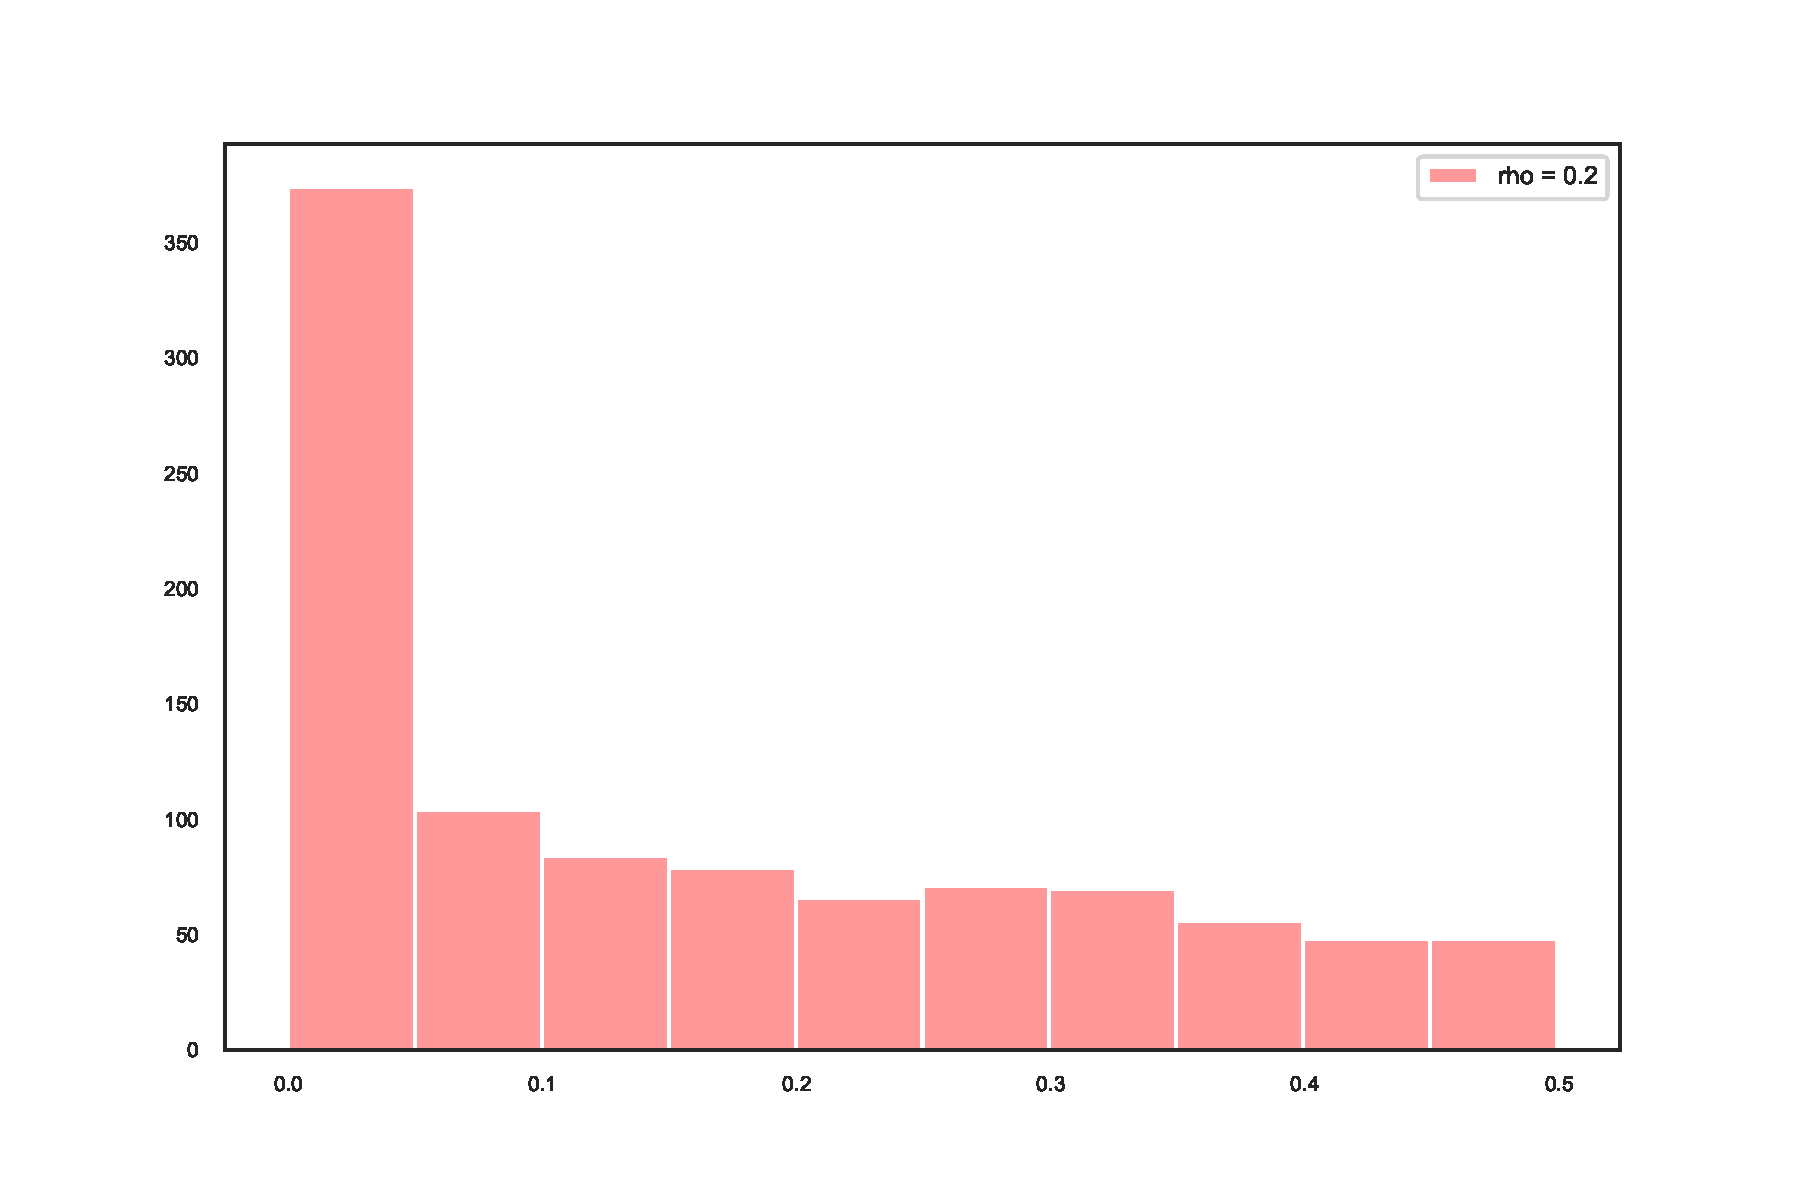
\includegraphics[width=0.8\textwidth]{sampler_task7_p2}}
\caption{Гистограма распределение p-value без поправок}
\label{sampler_task7_p2}
\end{figure}

\begin{figure}[h!]\center
{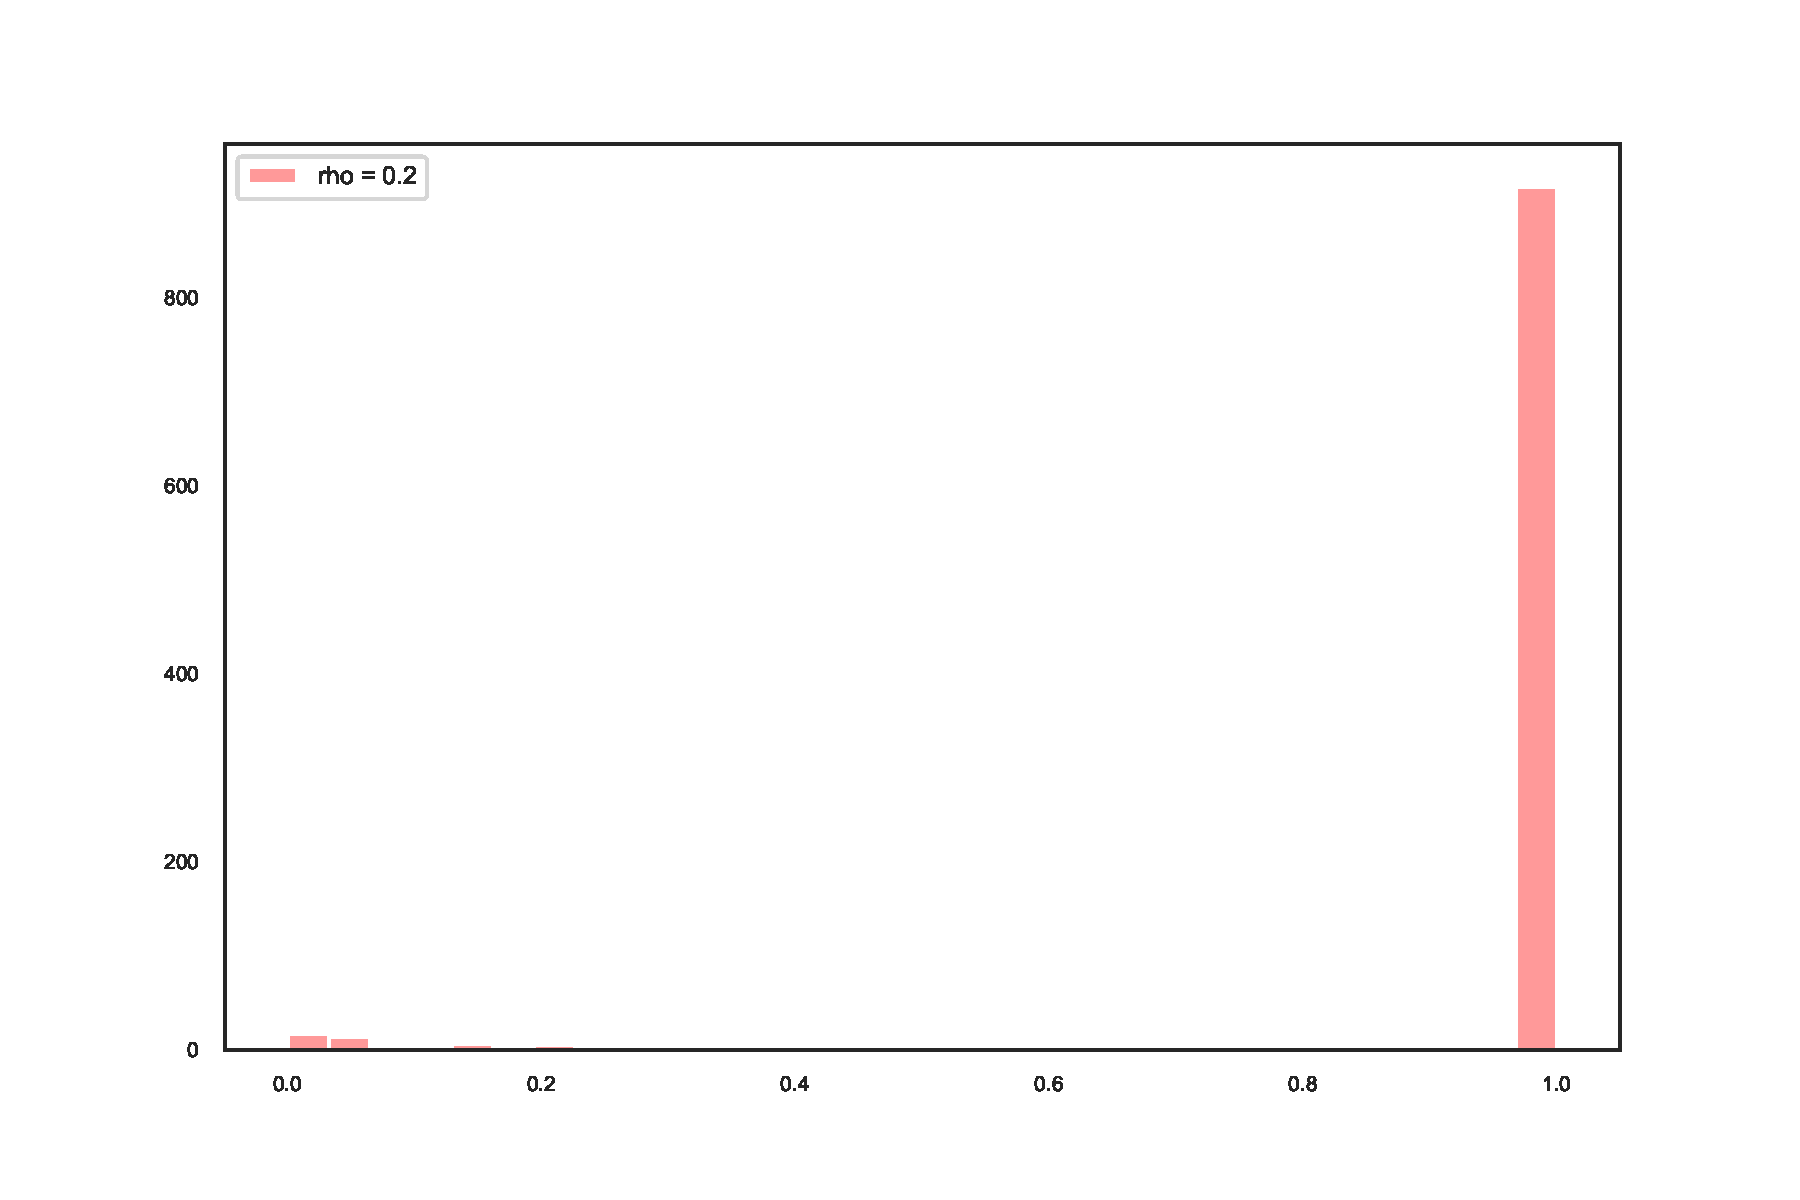
\includegraphics[width=0.8\textwidth]{sampler_task7_p3}}
\caption{Гистограма распределение p-value с Банферонии}
\label{sampler_task7_p3}
\end{figure}

\begin{figure}[h!]\center
{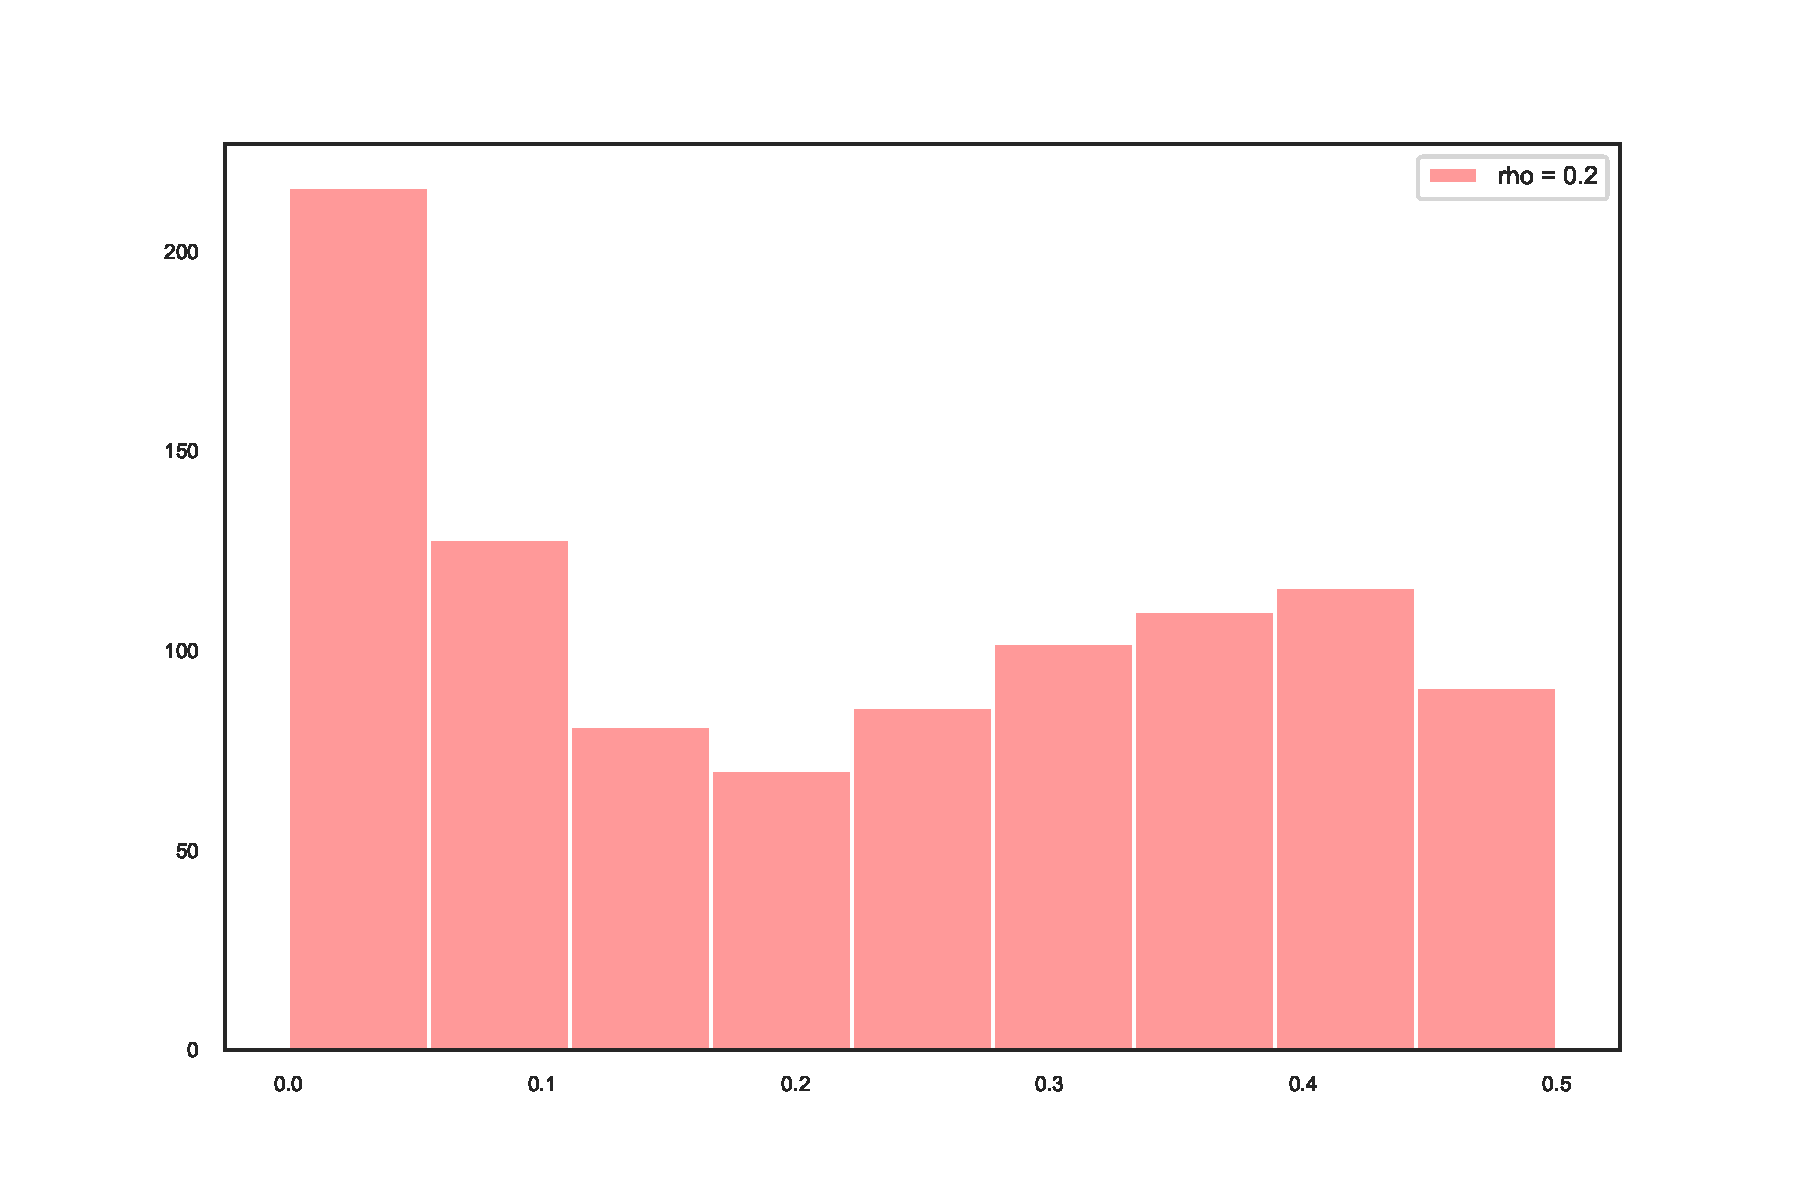
\includegraphics[width=0.8\textwidth]{sampler_task7_p4}}
\caption{Гистограма распределение p-value с Бенджамини-Хохберг}
\label{sampler_task7_p4}
\end{figure}

Распределение достигаемых уровней показаны на Рис.~[\ref{sampler_task7_p2},~\ref{sampler_task7_p3},~\ref{sampler_task7_p4}]

Для уровня значимости $\alpha = 0.05$ сравним результаты применения отсутствия поправки на на множественном тестирование и с использованием поправок Бонферони и Бенджамини-Хохберга. Результаты эксперимента показаны в таб.~\ref{table2}.

\begin{table}[h!]
\begin{center}
\begin{tabular}{|c|c|c|}
\hline
	Метод&Ложно отклоненные& Ложно принятые\\
	\hline
	Без поправки &  64 & 193 \\
	\hline
	Бонферони & 0 & 478\\
	\hline
	Бенджамини-Хохберга& 1 & 403\\
\hline
\end{tabular}
\end{center}
\caption{Для уровня значимости $\alpha = 0.05$}
\label{table2}
\end{table}

\end{document} 